\documentclass[12pt,a4paper,oneside]{report}
\usepackage[utf8]{inputenc}
\usepackage[english,russian]{babel}
\usepackage{amsmath}
\usepackage{commath}
\usepackage{amssymb}
\usepackage{array}
\usepackage{geometry}
\usepackage{sverb}
\usepackage{graphicx}
\usepackage{pdfpages}
\usepackage{hyperref} 
\usepackage{url}
\usepackage{titlesec, blindtext, color}
\usepackage{listings}
\usepackage{pgfplots}
\pgfplotsset{compat=newest}
\graphicspath{{../}}
\DeclareGraphicsExtensions{.pdf,.png,.jpg}
\usepackage{tabularx}
\usepackage{subcaption}
\usepackage{colortbl}
\usepackage{multirow}
\usepackage{longtable}
\usepackage{enumitem}
\usepackage{algorithm}
\usepackage{tikz}
\usepackage[noend]{algpseudocode}
\usepackage{float}
\definecolor{gray75}{gray}{0.75}
\definecolor{Blue}{HTML}{5D8AA8}
\newcommand{\hsp}{\hspace{20pt}}

\newcommand{\RomanNumeralCaps}[1]
{\MakeUppercase{\romannumeral #1}}

\newenvironment{conditions*}
{\par\vspace{\abovedisplayskip}\noindent
	\tabularx{\columnwidth}{>{$}l<{$} @{${}-{}$} >{\raggedright\arraybackslash}X}}
{\endtabularx\par\vspace{\belowdisplayskip}}

\newenvironment{conditions_eq*}
{\par\vspace{\abovedisplayskip}\noindent
	\tabularx{\columnwidth}{>{$}l<{$} @{${}={}$} >{\raggedright\arraybackslash}X}}
{\endtabularx\par\vspace{\belowdisplayskip}}

\setlength{\jot}{2ex}

\captionsetup{labelsep=period}

\addto\captionsrussian{\renewcommand{\figurename}{Рисунок}}



\geometry{pdftex, left = 2cm, right = 2cm, top = 2.5cm, bottom = 2.5cm}

% Для листинга кода:
\lstset{ %
	language=c++,                 % выбор языка для подсветки (здесь это С)
	basicstyle=\small\sffamily, % размер и начертание шрифта для подсветки кода
	numbers=left,               % где поставить нумерацию строк (слева\справа)
	numberstyle=\tiny,           % размер шрифта для номеров строк
	stepnumber=1,                   % размер шага между двумя номерами строк
	numbersep=5pt,                % как далеко отстоят номера строк от подсвечиваемого кода
	showspaces=false,            % показывать или нет пробелы специальными отступами
	showstringspaces=false,      % показывать или нет пробелы в строках
	showtabs=false,             % показывать или нет табуляцию в строках
	frame=single,              % рисовать рамку вокруг кода
	tabsize=2,                 % размер табуляции по умолчанию равен 2 пробелам
	captionpos=b,              % позиция заголовка вверху [t] или внизу [b] 
	breaklines=true,           % автоматически переносить строки (да\нет)
	breakatwhitespace=false, % переносить строки только если есть пробел
	escapeinside={\#*}{*)}   % если нужно добавить комментарии в коде
}



\titleformat{\chapter}[hang]{\Huge\bfseries}{\thechapter.\textcolor{black}\hsp}{0pt}{\Huge\bfseries}
\setcounter{tocdepth}{4} % фикс переноса 
\begin{document}
	\thispagestyle{empty}
	\noindent \begin{minipage}{0.15\textwidth}
		
\includegraphics[width=\linewidth]{b_logo}
	\end{minipage}
	\noindent\begin{minipage}{0.9\textwidth}\centering
		\textbf{Министерство науки и высшего образования Российской Федерации}\\
		\textbf{Федеральное государственное бюджетное образовательное учреждение высшего образования}\\
		\textbf{«Московский государственный технический университет имени Н.Э.~Баумана}\\
		\textbf{(национальный исследовательский университет)»}\\
		\textbf{(МГТУ им. Н.Э.~Баумана)}
	\end{minipage}
	\noindent\rule{18cm}{3pt}
	\newline\newline
	\noindent ФАКУЛЬТЕТ $\underline{\textbf{«ИНФОРМАТИКА И СИСТЕМЫ УПРАВЛЕНИЯ»}}$ \newline\newline
	\noindent КАФЕДРА $\underline{\textbf{«ПРОГРАММНОЕ ОБЕСПЕЧЕНИЕ ЭВМ И ИНФОРМАЦИОННЫЕ }}$\newline\newline
	$\underline{\textbf{ТЕХНОЛОГИИ»(ИУ7)}}$\newline\newline
	\noindent НАПРАВЛЕНИЕ ПОДГОТОВКИ $\underline{\textbf{09.03.04 ПРОГРАММНАЯ ИНЖЕНЕРИЯ}}$\newline\newline\newline\newline\newline\newline\newline
	\begin{center}
		\begin{flushright}
			\Large\textbf{РАСЧЕТНО-ПОЯСНИТЕЛЬНАЯ ЗАПИСКА}\newline
			\Large\textbf{К КУРСОВОМУ ПРОЕКТУ}\newline
			\Large\textbf{НА ТЕМУ:}\newline
			\Large\textbf{«Построение реалистического изображения из трехмерных геометрических объектов»}\newline
		\end{flushright}
	\end{center}
	\noindent\textbf{} $\underline{\text{}}$\newline\newline\newline\newline
	
	\begin{tabular}{lcp{5em}lp{2em}l}
		\noindent\textbf{Студент} &  $\underline{\text{ИУ7-52Б~~}}$ &             &\hspace{1cm} & & $\underline{\text{Д.В. Анцибор}}$ \\\cline{4-3}
		& (Группа) & &(Подпись,дата)  & & (И.О.Фамилия) \\
		& & & & &\\
		\noindent\textbf{Руководитель} & \textbf{курсового} &  \textbf{проекта}&\hspace{1cm} & &$\underline{\text{А.С. Ваулин~}}$ \\\cline{4-3} 
		&  & & (Подпись,дата)  & &(И.О.Фамилия) \\
	\end{tabular}
	
	\begin{center}
		\vfill
		Москва, 2020
	\end{center}
	\newpage
	
	\renewcommand*\contentsname{Содержание}
	\tableofcontents
	\setcounter{page}{1}
	\newpage
	
	\addcontentsline{toc}{chapter}{Введение}
	\chapter*{Введение}
	
	%\Large
	\quad Компьютерная графика -- область деятельности, в которой компьютерные технологии используются для создания изображений, а также обработки визуальной информации. 
	
	 В настоящее время в компьютерной графике большое внимание уделяется алгоритмам получения реалистичных изображений. Так как данные алгоритмы должны учитывать множество физических явлений, таких как преломление, различные виды отражения и т.п. -- они являются довольно требовательными к ресурсам системы. Сложность вычислений напрямую зависит от требований, предъявляемых к реалистичности изображения, степени его проработанности. Стремление к созданию наиболее реалистичного изображения становится трудно выполнимым при моделировании динамических сцен, в которых требуется поддержание высокой частоты кадров. 
	
	
	 Для успешного решения поставленной задачи необходимо произвести её анализ, декомпозицию. Решение необходимо написать на выбранном языке программирования и спроектировать удобный для пользователя интерфейс. 
	
	 Целью данной работы является проведение исследований алгоритмов, применяемых для построения реалистического изображения, а также алгоритмов, позволяющих работать с камерой наблюдателя, удалять невидимые поверхности, создавать освещение и проецировать результат на экран.
	
	 \textbf{Для достижения поставленной цели необходимо решить следующие задачи: } 
	
	\begin{itemize}
		\item провести анализ существующих алгоритмов удаления невидимых линий и поверхностей, закраски, текстурирования, а также моделей освещения и выбрать из них подходящие для выполнения проекта;
		\item реализовать выбранные алгоритмы и структуры данных;
		\item разработать программное обеспечение, которое позволит отобразить трехмерную сцену;
		\item реализовать интерфейс программного модуля;
		\item провести исследования на основе разработанной программы. 
		
	\end{itemize}

	Результатом выполнения работы является программное обеспечение для создания графических сцен из готовых трехмерных моделей и их визуализации с учетом выбранной текстуры или цвета, а также оптических эффектов отражения, преломления, прозрачности, блеска. 
	
 	\chapter {Aналитический раздел}
 	
 	 \quad Задачу отрисовки сцены можно разбить на составные задачи, которые требуется решить для получения финального результата, а именно: выбор способа представления модели, перевод координат модели из пространства объекта в пространство экрана, удаление невидимых линий, растеризация, добавление освещения, проведение преобразований над объектом, перемещение камеры. В случае с генерацией реалистического изображения стоит использовать алгоритм обратной трассировки лучей, который позволяет добиться получения красивой картинки.
 	  
 		 
 	\section{Описание модели трехмерного объекта в сцене}
 	
 	 \quad В компьютерной графике существует множество способов задания трехмерных объектов, но в данной работе было необходимо выбрать такой способ, который позволил бы воспринимать объекты объемными, накладывать текстуру на них. С учетом этих целей модель можно представить в виде:
 	\begin{itemize}
 		\item геометрического примитива;
 		\item полигональной сетки.
 	\end{itemize}

	\subsection{Модель как геометрический примитив}
	 \quad Примитив, как правило, может быть описан процедурой, которая принимает некоторые значения параметров, например, для построения сферы достаточно знать её радиус и положение центра. В качестве таких примитивов могут выступать тела с простой формой: куб, цилиндр, призма, пирамида, сфера, конус.\\
	
	К плюсам таких моделей можно отнести:
	\begin{itemize}
		\item простоту построения, что увеличивает скорость работы программы;
		\item минимальное, по сравнению с другими способами представления моделей, количество ключевой информации, необходимой для их отрисовки.
	\end{itemize}
	
	В то же время к минусам относится:
	\begin{itemize}
		\item данные модели могут описывать только простейшие объекты;
		\item наложение текстуры затруднительно.
	\end{itemize}

	\subsection{Модель как полигональная сетка}
	 \quad Полигональная сетка — это совокупность вершин, рёбер и граней, которые определяют форму многогранного объекта в трёхмерной компьютерной графике и объёмном моделировании. Гранями обычно являются треугольники, четырёхугольники или другие простые выпуклые многоугольники (полигоны), так как это упрощает рендеринг, но сетки могут также состоять и из наиболее общих вогнутых многоугольников, или многоугольников с отверстиями.
	 
	 Данный способ задания модели является достаточно универсальным, так как с его помощью можно задать объект любой формы. В качестве полигона может быть выбран любой многоугольник, однако чаще всего используется треугольник. Так как любой другой многоугольник можно разбить на треугольники.
	
	 От количества полигонов в модели зависит то, насколько детально-проработанной она будет выглядеть, соответственно чем их больше, тем лучше выглядит модель, однако с ростом их числа растет время, которое программа затрачивает на отрисовку всех моделей в сцене. Благодаря тому, что полигоны задают плоскости, можно изменять нормали для достижения необходимых эффектов иммитации неровностей поверхности, а также при создании модели указать текстурные координаты, то есть то, как изображение будет накладываться на модель.
	
	 В отличие от примитивов, создание такой модели требует проведения предварительной работы, так как необходимо явно указать как будет выглядеть полигональная сетка, задать текстурные координаты.
	
	\subsection{Выводы}
	 \quad После анализа особенностей представления обоих вариантов в качестве способа задания модели была выбрана полигональная сетка, так как процесс наложения тексктуры для таких объектов наиболее прост, а также это дало возможность добавлять те объекты в сцену, которые нельзя или трудно задать параметрически.
	
	\section{Алгоритмы построения трехмерного изображения}
	
	\subsection{Алгоритм Варнока}
	
	 \quad Алгоритм Варнока является одним из примеров алгоритма, основанного на разбиении картинной плоскости на части, для каждой из которых исходная задача может быть решена достаточно просто\cite{f}. 
	
	 В пространстве изображения рассматривается окно и решается вопрос о том, пусто ли оно, или его содержимое достаточно просто для визуализации. Если это не так, то окно разбивается на фрагменты до тех пор, пока содержимое фрагмента не станет достаточно простым для визуализации или его размер не достигнет требуемого предела разрешения. В последнем случае информация, содержащаяся в окне, усредняется, и результат изображается с одинаковой интенсивностью или цветом. В оригинальной версии алгоритма каждое окно разбивалось на четыре одинаковых подокна. 
	
	 Многоугольник, входящий в изображаемую сцену, называют:
	\begin{itemize}
		\item внешним, если он целиком находится вне окна – Рисунок 1.1a;
		\item внутренним, если он целиком расположен внутри окна – Рисунок 1.1b;
		\item пересекающим, если он пересекает границу окна – Рисунок 1.1c;
		\item охватывающим, если окно целиком расположено внутри него – Рисунок 1.1.
	\end{itemize}
	
	\begin{figure}[h]
		\centering
		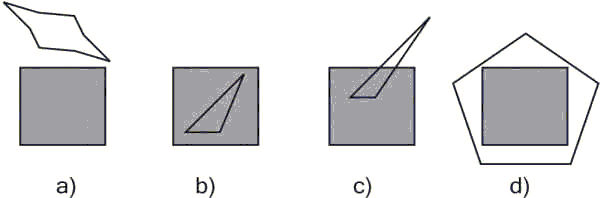
\includegraphics[scale=0.6]{varnok}
		\caption{Примеры расположения окна}
	\end{figure}

	Достоинством алгоритма Варнока является учет когерентности, из-за чего скорость его работы повышается при увеличении размеров однородных областей изображения. К недостаткам алгоритма можно отнести невозможность передачи зеркальных эффектов и преломления света, а также несовершенство способа разбиения изображения – в сложных сценах число разбиений может стать очень большим, что приведет к потере скорости.
	
	\subsection{Алгоритм Вейлера-Азертона}
	\quad Алгоритм Вейлера-Азертона является попыткой минимизировать количество шагов в алгоритме Варнока путём разбиения окна вдоль границ многоугольника. Метод работает с проекциями граней на картинную плоскость.
	
	Алгоритм выполняет следующую последовательность действий:
	\begin{enumerate}
		\item Предварительная сортировка по глубине (для формирования списка приблизительных приоритетов).
		\item Отсечение по границам ближайшего к наблюдателю многоугольника (в качестве отсекателя используется копия первого многоугольника из списка приблизительных приоритетов. Отсекаться будут все многоугольники в этом списке, включая первый. Формируется 2 списка – внутренний и внешний).
		\item Удаление многоугольников внутреннего списка, которые экраниру-ются отсекателем.
		\item Если глубина многоугольника из внутреннего списка больше, чем Zmin отсекателя, то такой многоугольник частично экранирует отсекатель. Нужно рекурсивно разделить плоскость, используя многоугольник, нарушивший порядок, в качестве отсекателя (нужно использовать копию исходного многоугольника, а не остаток после предыдущего отсечения). Отсечению подлежат все многоугольники из внутреннего списка.
		\item По окончании отсечения или рекурсивного разбиения изображаются многоугольники из внутреннего списка (те, которые остались после удаления всех экранируемых на каждом шаге многоугольников – остаются только отсекающие многоугольники).
		\item Работа продолжается с внешним списком (шаги 1-5).
	\end{enumerate}
	
	 Если многоугольники пересекаются, то для корректной работы данного алгоритма нужно плоскость одного разбить другим на две части. Эффективность алгоритма Вейлера-Азертона, как и алгоритма Варнока, зависит от эффективности разбиений. В дальнейшем этот алгоритм был распространен на сплайновые поверхности. К достоинствам алгоритма можно отнести скорость работы, учет когерентности изображения. Недостатками алгоритма является сложность реализации.
	
	\subsection{Z-буфер}
	 \quad Это алгоритм, работающий в пространстве изображения, как показано на рисунке 1.2. Буфер кадра используется для запоминания интенсивности каждого пиксела в пространстве изображения, z-буфер — это отдельный буфер глубины, используемый для запоминания координаты z или глубины каждого видимого пиксела в пространстве изображения. 

	\begin{figure}[h]
		\centering
		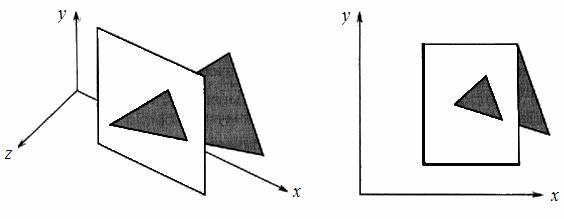
\includegraphics[scale=0.6]{z-buffer}
		\caption{Пример алгоритма с использованием Z-буфера}
	\end{figure}
	
	 В процессе работы значение z каждого пиксела, который нужно занести в буфер кадра, сравнивается с глубиной уже занесенного в z-буфер пиксела. Если новый пиксел расположен впереди пиксела, находящегося в буфере кадра, то новый пиксел заносится в этот буфер и производится корректировка z-буфера новым значением z. 
	
	 К достоинствам алгоритма, использующего z-буффер можно отнести простоту реализации, а также отсутствие предварительной сортировки элементов сцены. Недостатками алгоритма являются трудоёмкость реализации эффектов прозрачности, а также перерасход по памяти -- алгоритм предполагает хранение двух двумерных массивов, размер которых увеличивается с увеличением размеров изображения.
	
	
 	\subsection{Алгоритм художника}
 	\quad Простейший программный вариант решения «проблемы видимости» в трехмерной компьютерной графике\cite{s}.
 	Название «алгоритм художника» относится к технике, используемой многими живописцами: сначала рисуются наиболее удалённые части сцены, потом части, которые ближе. Постепенно ближние части начинают перекрывать отдаленные части более удалённых объектов. Задача программиста при реализации алгоритма художника -- отсортировать все полигоны по удалённости от наблюдателя и начать выводить, начиная с более дальних. 
 	
 	 Алгоритм не позволяет получить корректную картину в случае взаимно перекрывающихся полигонов. В этом случае полигоны накладываются друг на друга таким образом, что невозможно определить, в каком порядке их следует рисовать. 	
 	Второй распространённой проблемой является то, что система прорисовывает также области, которые впоследствии будут перекрыты, на что тратится лишнее процессорное время.
 	
 	\subsection{Алгоритм обратной трассировки лучей}
 	
 	 \quad Алгоритм обратной трассировки лучей выглядит следующим образом: из камеры через каждый пиксел изображения испускается луч и находится точка его пересечения с поверхностью сцены. Лучи, выпущенные из камеры, называют первичными. 
 	
 	 Пусть, первичный луч пересекает некий объект 1 в точке H1, как показано на рисунке 1.3.
 	
 	\begin{figure}[H]
 		\centering
 		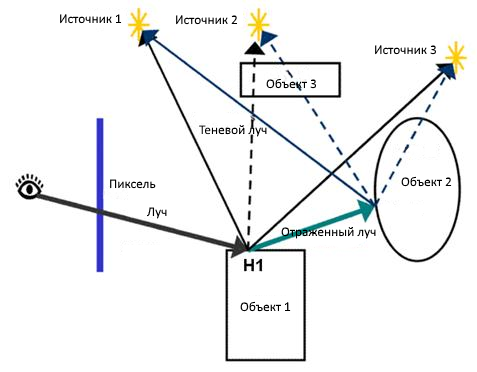
\includegraphics[scale=0.8]{ray}
 		\caption{Алгоритм обратной трассировки лучей}
 	\end{figure}
 
 	 Далее необходимо определить для каждого источника освещения, видна ли из него эта точка. Тогда в направлении каждого точечного источника света испускается теневой луч из точки H1. Это позволяет определить, освещается ли данная точка конкретным источником. Если теневой луч находит пересечение с другими объектами, расположенными ближе к точке H1, чем источник света, значит, точка H1 находится в тени от этого источника и освещать ее не надо, иначе освещение рассчитывается по некоторой локальной модели. Освещение со всех видимых (из точки H1) источников света складывается. Далее, если материал объекта 1 имеет отражающие свойства, из точки H1 испускается отраженный луч и для него вся процедура трассировки рекурсивно повторяется. Аналогичные действия должны быть выполнены, если материал имеет преломляющие свойства.
 
 	 Техника рендеринга с трассировкой лучей отличается высоким реализмом получаемого изображения\cite{four}. Она позволяет воссоздавать тени, отражения и преломления света. Алгоритм трассировки позволяет выполнять вычисления параллельно. Также обеспечивется отсечение невидимых поверхностей, перспектива.
 	
 	 Недостатком метода обратного трассирования является производительность. Трассировка лучей каждый раз начинает процесс определения цвета пикселя заново, рассматривая каждый трассируемый луч в отдельности.
 	
 	\subsection {Выводы}
 	 \quad Для создания реалистичного изображения лучше всего подходит алгоритм обратной трассировки лучей, однако из-за низкой производительности алгоритм фактически неприменим к созданию сцены в реальном времени. Поэтому в программе будет предусмотрено два режима работы. В первом режиме пользователь сможет добавлять новые объекты, редактировать их размер, положение, выбирать цвет и текстуру, на данном этапе важна скорость, поэтому в качестве алгоритма отсечения невидимых линий и поверхностей был выбран алгоритм z-буфера. Во втором режиме программа должна будет строить реалистичное изображение, учитывать тени, прозрачность, отражение объектов, поэтому в этом режиме будет использоваться алгоритм обратной трассировки лучей, как позволяющий достичь наибольшей реалистичности построенного изображения.
 	
 	\section {Анализ алгоритмов наложения текстур на объекты трёхмерной сцены}
 	\subsection{Аффинное текстурирование}
 	 \quad Этот метод текстурирования основан на приближении u, v линейными функциями, где u, v – координаты текстуры. Пусть u - линейная функция, $u = k_1 \times sx + k_2 \times sy + k_3$, где sx, sy - координаты принадлежащие проекции текстурируемого треугольника. Можно посчитать $k_1$, $k_2$, $k_3$ исходя из того, что в вершинах грани u, v известны -- это даст три уравнения, из которых находятся эти коэффициенты. Однако в таком случае вычисление цвета пикселя получается медленным. Оптимизацией данного подхода является расчет начальных значений координат текстур для каждого полигона, а затем билинейная интерполяция значений x и y текстуры. Основным недостатком этого метода является игнорирование координаты z, вследствие чего данные искажаются, и текстура накладывается нереалистично.
 	
 	\subsection{Перспективно-корректное текстурирование}
 	\quad Этот метод основан на приближении u, v кусочно-линейными функциями. При отрисовке каждая сканирующая строка разбивается на части, в начале и конце каждого куска считаются точные значения u, v, а в каждой части они интерполируется линейно.
 	
 	 Точные значения u и v можно считать по формулам точного текстурирования, но обычно используют более простой путь. Он основан на том факте, что значения 1/Z, u/Z и v/Z зависят от sx, sy линейно. Таким образом, достаточно для каждой вершины посчитать 1/Z, u/Z, v/Z и линейно их интерполировать -- точно так же, как интерполируются u и v в аффинном текстурировании. Причем, поскольку эти значения зависят от sx, sy строго линейно, то интерполяция дает не приближенные результаты, а точные.
 	
 	Сами же точные значения u, v считаются, как:
 	
 	%\Large
 	\begin{equation}
 	u = (u / z) / (1 / z),
 	v = (v / z) / (1 / z)
 	\end{equation}
 	
 	\subsection{Выводы}
 	 \quad Наиболее приемлемой является перспективно-корректная реализация, поскольку в ее основе лежит точное текстурирование, что делает ее результаты более приближенными к действительным, нежели у аффинной, к тому же она учитывает перспективу изображения. 
 	
 	\section {Алгоритмы закраски треугольников}
 	\subsection{Алгоритмы со списком рёберных точек}
 	 \quad Этот алгоритм подходит только для тех случаев, когда закрашиваемая область может быть задана в виде многоугольника. Предполагается, что  работа проводится с многоугольником с вершинами P1,P2,…,PN и требуется отобразить его на экране вместе со всеми внутренними точками. Для удобства принимается, что каждое ребро многоугольника задаётся координатами его концов x1,y1 и x2,y2 (при этом $y2 \geqslant y1$). Также считается, что координата x возрастает при движении слева направо, а координата y при движении сверху вниз(рисунок 1.4).
 	Подавляющее большинство алгоритмов растеризации многоугольников основаны на следующем предположении: любая секущая прямая пересекает границу многоугольника чётное число раз. Это утверждение неверно только в двух случаях:
 	\begin{itemize}
 		\item когда секущая прямая содержит ребро;
 		\item когда секущая прямая содержит вершину, а смежные рёбра лежат по одну сторону от секущей прямой.
 	\end{itemize}
 	
 	Эти два случая довольно легко обнаружить, поэтому при рассмотрении алгоритмов растеризации многоугольников считается, что приведённое выше предположение всегда верно.
 	
 	\begin{figure}[H]
 		\centering
 		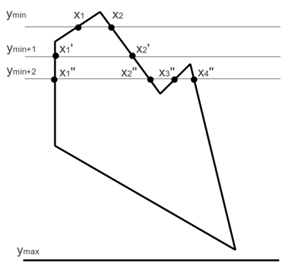
\includegraphics[scale=0.8]{poligon_intersect_line}
 		\caption{Пересечение многоугольника сканирующей строкой}
 	\end{figure}
 
 	 Алгоритм, основанный на работе со списком рёберных точек, состоит из трёх основных этапов:
 	\begin{enumerate}
 		\item На первом этапе растеризуются все негоризонтальные рёбра многоугольника. Для каждого значения y составляется список x-координат, закрашенных при растеризации.
 		\item На втором этапе для каждого значения y списки упорядочиваются по возрастанию.
 		\item На третьем этапе для каждого y заполняются все полученные отрезки.
 	\end{enumerate}
 	
 	 Преимущество этого алгоритма в том, что каждый пиксель обрабатывается строго один раз. Таким образом можно утверждать, что этот алгоритм подходит для устройств, где доступ к видео-памяти занимает сравнительно много времени.
 	Существует модификация данного алгоритма, оптимизированная по расходу памяти. В ней на каждом шаге обрабатываются только те рёбра, которые пересекаются с текущей линией развёртки.
 	
 	\subsection{Алгоритм XOR для граней}
 	 \quad Метод XOR для граней описывается следующим простым алгоритмом: для каждого ребра в многоугольнике инвертируются цвета всех пикселов, расположенных правее этого ребра, при этом порядок обхода рёбер не имеет значения. На рисунке 1.5 приведены шаги этого алгоритма (движение по часовой стрелке):
 	
 	\begin{figure}[H]
 		\centering
 		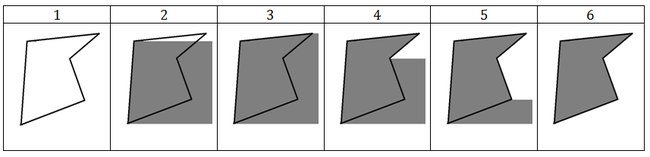
\includegraphics[scale=0.7]{fill_poly_001}
 		\caption{Алгоритм XOR для граней}
 	\end{figure}
 	
 	 Недостаток этого алгоритма – высокие временные затраты, так как некоторые пикселы обрабатываются более одного раза. Кроме того, чем больше расстояние от изображения до правой границы области экрана, тем больше будет совершено лишних операций.
 	
 	\subsection{Алгоритм разделения}
 	 \quad Схематично алгоритм можно описать следующим образом:
 	\begin{enumerate}
 		\item Треугольник разбивается на две части вертикальной линией, проходящей через среднюю точку(рисунок 1.6).
 		\item Каждый из двух полученных треугольников растеризуется по отдельности. Причем в процессе растеризации связность растеризуемых линий (сторон треугольника) не обеспечивается(рисунок 1.7).
 		\item При получении координат текущих точек горизонтальный отрезок между ними заполняется.
 	\end{enumerate}
 
	\begin{figure}[H]
		\centering
		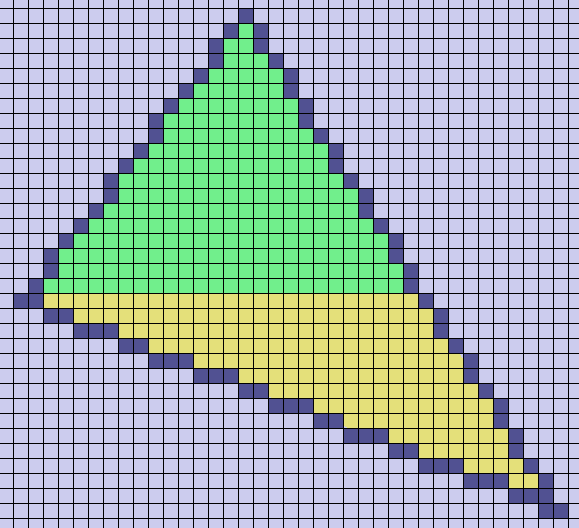
\includegraphics[scale=0.4]{11_triangle}
		\caption{Разделение треугольника на 2 части}
	\end{figure}

	\begin{figure}[H]
		\centering
		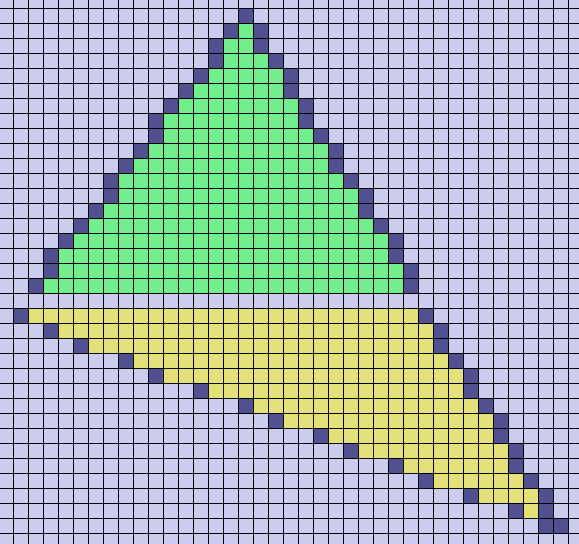
\includegraphics[scale=0.4]{11_triangle_yrast}
		\caption{Раздельное закрашивание двух треугольников}
	\end{figure}

	 Данный алгоритм работает достаточно быстро, однако вызывает трудности в процессе интепролирования различных атрибутов полигона - нормалей, цвета вершин, координат текстур.
	
	\subsection{Алгоритм заполнения треугольника с использованием барицентрических координат}
	  \quad Барицентрические координаты - это координаты, в которых точка треугольника описывается как линейная комбинация вершин (формально, подразумевая, что точка является центром масс треугольника, при соответствующем весе вершин). Чаще всего используют нормализованный вариант -- т.е. суммарный вес трех вершин равен единице:
	\begin{equation}
	\begin{gathered}
	p = b_0  v_0 + b_1   v_1 + b_2  v_2\\
	b_0 + b_1 + b_2 = 1
	\end{gathered}
	\end{equation}
	
	
	 У этой системы координат так же есть очень полезное свойство, которое позволяет их вычислять: барицентрические координаты равны отношению площадей треугольников, к общей площади треугольника (рисунок 1.8).
	\begin{figure}[h]
		\centering
		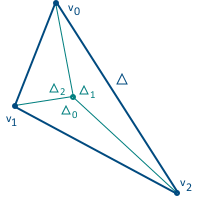
\includegraphics[scale=0.7]{bary}
		\caption{Представление барицентрических координат}
	\end{figure}

	\begin{equation}
	\begin{aligned}
	b_0 &= \frac{\delta_0}{\delta}\\
	b_1 &= \frac{\delta_1}{\delta}\\
	b_2 &= 1 - b_1 - b_0
	\end{aligned}
	\end{equation}
	
	 Третья координата может вычисляться не через площади треугольников, поскольку сумма трех координат равна единице -- фактически, мы имеем только две степени свободы.
	
	 Главной особенностью данных координат является то, что с их помощью можно интерполировать значение любого атрибута в произвольной точке треугольника: значение атрибута в заданной точке треугольника равно линейной комбинации барицентрических координат и значений атрибута в соответствующих вершинах:
	
	\begin{equation}
	T = b_0 T_0 + b_1 T_1 + b_2 T_2
	\end{equation}
	
	 Для коррекции перспективы используют другую формулу -- сначала вычисляют интерполированное значение $\frac{T}{z}$, затем интерполированное значение $\frac{1}{z}$, и затем делят их друг на друга, чтобы получить итоговое значение $T$ с учетом перспективы:
	
	\begin{equation}
	\begin{gathered}
	\frac{T}{z} = \frac{T_0}{z}  b_0 + \frac{T_1}{z}  b_1 + \frac{T_2}{z}  b_2\\
	\frac{1}{z} = \frac{1}{z_0}  b_0 + \frac{1}{z_1}  b_1 + \frac{1}{z_2}  b_2\\
	T = \frac{\frac{T}{z}}{\frac{1}{z}}
	\end{gathered}
	\end{equation}
	
	 Сам же алгоритм закраски с использованием данных координат достаточно прост:
	\begin{enumerate}
		\item Для начала надо найти минимальный по площади прямоугольник, который бы создержал в себе данный треугольник.
		\item Далее для каждой строки прямоугольника проводим его сканирование слева направо.
		\item Для каждого выбранного пикселя находим его барицентрические координаты.
		\item Если значение каждой из них находится в отрезке от 0 до 1 и их сумма не превышает 1, то закрашиваем пиксель.
	\end{enumerate}

	\subsection{Выводы}
	 \quad Алгоритм с использованием барицентрических координат оказался сам эффективным и легко реализуемым из выше перечисленных, а также предоставил возможность корректно интерполировать атрибуты треугольника, что было бы затруднительно или невозможно при использовании других алгоритмов.
	
	\section{Описание трехмерных преобразований}
	
	\subsection{Способы хранения и обработки декартовых координат}
	 \quad Координаты можно хранить в форме вектор-столбца [x, y, z]. Однако в этом случае неудобно применять преобразования поворота, так как такой вектор нельзя умножить на соответствующие квадратные матрицы трансформации размерности четыре на четыре. Целесообразнее использовать вектор-столбцы размерности четыре -- [x,y,z,w], где координата w = 1. Преобразования координат выполняются умножением слева преобразуемого вектора-строки на соответствующую матрицу линейного оператора.
	
	\subsection{Преобразование трехмерного пространства в двумерное пространство экрана}
	 \quad Несмотря на то, что мы живем в трехмерном мире (то есть у любого объекта можно измерить длину, ширину, высоту, что позволяет воспринимать любой объект в окружающем мире как нечто объемное) пространство экрана компьютера обладает только двумя из трех измерений, а именно шириной и высотой. Трехмерное пространство описывается тремя единичными ортогональными векторами. То есть если, например, взять совершенно случайный объект реального мира и мысленно как-то расположить трехмерную систему координат относительно этого объекта, то каждая точка на его поверхности будет однозначно описана. 
	
	 В тоже время экран компьютера имеет лишь две координаты и состоит из пикселей, изменяя цвет которых получается итоговое изображение. Каждый пиксель может быть однозначно задан двумя координатами х и у, в силу чего возникает проблема изображения трехмерного объекта на экране с сохранением эффекта объемности.
	
	Обычно многие графические программы делают это путем применения четырех преобразований (рисунок 1.9):
	\begin{enumerate}
		\item Перевод объекта из собственного пространства в мировое.
		\item Перевод объекта из мирового пространства в пространство камеры.
		\item Проекция всех точек из пространства камеры во все видимые точки, где координаты x, y, z находятся в диапазоне [-w;w], а w в диапазоне [0;w].
		\item Масштабирование точек, полученных после предыдущего преобразования на картинку необходимого разрешения.
	\end{enumerate}

	\begin{figure}[H]
		\centering
		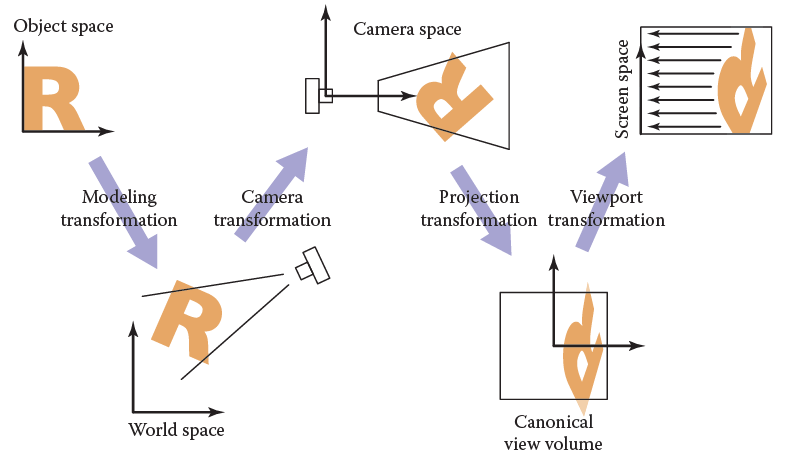
\includegraphics[scale=0.7]{spaces}
		\caption{Последовательность трансформаций, которые переводят объект из собственного пространства в пространство экрана компьютера}
	\end{figure}

	 Для выполнения этих этапов используют матрицы преобразований. Процесс обычно строится следующим образом:
	\begin{enumerate}
		\item Вычисляются все необходимые матрицы.
		\item Вычисленные матрицы перемножаются.
		\item Вектор-строка, описывающий положение точки в пространстве, умножается на результирующую матрицу.
	\end{enumerate}		
	
	\subsection{Матрицы аффинных преобразований декартовых координат}
	\begin{enumerate}
		\item Сдвиг точки на dx, dy, dz по координатным осям (рисунок 1.10).
		\begin{figure}[H]
			\centering
			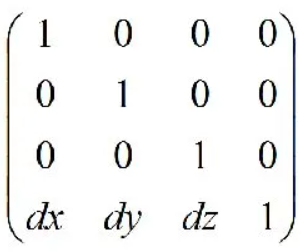
\includegraphics[width = .5\linewidth]{translation}
			\caption{Сдвиг точки на dx, dy, dz по координатным осям}
		\end{figure}
		
		\item Масштабирование относительно начала координат с коэффициентами sx, sy, sz (рисунок 1.11).
		\begin{figure}[H]
			\centering
			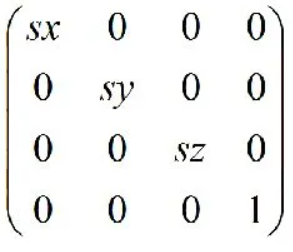
\includegraphics[width = .5\linewidth]{scale}
			\caption{Масштабирование относительно начала координат с коэффициентами sx, sy, sz}
		\end{figure}
	
		\item Поворот относительно осей x, y, z на угол $\alpha$ (рисунок 1.12).
		\begin{figure}[H]
			\centering
			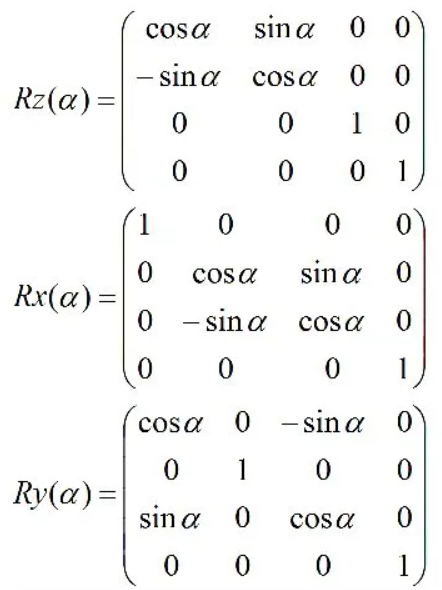
\includegraphics[width = .5\linewidth]{rotation}
			\caption{Поворот относительно осей x, y, z на угол $\alpha$}
		\end{figure}
	
	\end{enumerate}

	\subsection{Кватернионы}
	 \quad Кватернионы расширяют понятие вращения в трёх измерениях на вращение в четырёх измерениях и позволяют выполнить плавное и непрерывное вращение. Кватернионы определяются четырьмя действительными числами [x y z w]. Они вычисляются из комбинации оси и угла вращения. 
	
	 Пусть ось имеет координаты  (ox, oy, oz), а угол равен $\alpha$, тогда кватернион хранится в виде:
	\begin{equation}
	\begin{gathered}
	X = ox \times \sin(\frac{\alpha}{2})\\
	Y = oy  \times \sin(\frac{\alpha}{2})\\
	Z = oz  \times  \sin(\frac{\alpha}{2})\\
	W = \cos(\frac{\alpha}{2})
	\end{gathered}
	\end{equation}
	
	 C помощью кватернионов можно повернуть объект вокруг любой оси на заданный угол. Для того, чтобы применить несколько операций поворота последовательно, достаточно перемножить соответствующие кватернионы между собой. 
	
	\subsection{Преобразования трехмерной сцены в пространство камеры}
	 \quad Для того, чтобы преобразовать сцену в пространство камеры нужно умножить каждую вершину всех полигональных моделей на матрицу камеры (рисунок 1.13). Сама камера задается набором следующих атрибутов: положение центра камеры в мировом пространстве, вектора направления взгляда, направления верха камеры.
	
	\begin{figure}[H]
		\centering
		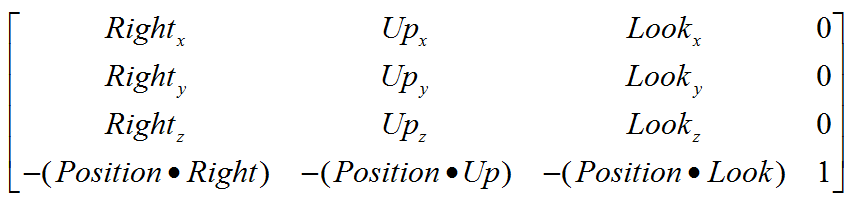
\includegraphics[scale=0.6]{view_matrix}
		\caption[LookAt матрица]
		{LookAt матрица \par где:\\
		Look -- координаты точки в пространстве, на которую смотрит камера, \\
		Up -- вектор, который указывает куда смотрит верх камеры,\\
		Right -- ортогональный вектор к векторам направления взгляда и вектору направления верха камеры\\
	}
	\end{figure}

	\subsection{Матрица перспективной проекции}
	 \quad После перехода в пространство камеры следует умножить каждую вершину всех полигональных моделей на матрицу проекции (рисунок 1.14). Матрица проекции отображает заданный диапазон усеченной пирамиды в пространство отсечения, и при этом манипулирует w-компонентой каждой вершины таким образом, что чем дальше от наблюдателя находится вершина, тем больше становится это w-значение. После преобразования координат в пространство отсечения x, y попадают в диапазон от -w до w , а вершина z от 0 до w (вершины, находящиеся вне этого диапазона, отсекаются).
	
	\begin{figure}[H]
		\centering
		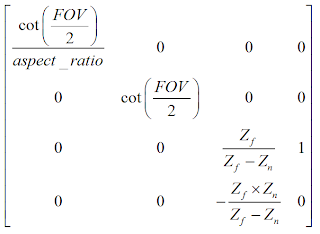
\includegraphics[scale=0.6]{projection_matrix}
		\caption[Матрица перспективной проекции]{
			Матрица перспективной проекции \par где:\\
			aspect ratio - отношение ширины изображения к его высоте, \\
			FOV -- угол обзора камеры,\\
			$Z_n$ -- координата z ближней к камере плоскости отсечения пирамиды видимости,\\
			$Z_f$ -- координата z дальней от камеры плоскости отсечения пирамиды видимости
		}
	\end{figure}

	 После перевода в пространство камеры, все координаты необходимо спроецировать на одну плоскость путем деления на координату z. Стоит отметить, что после применения умножения вектора координат на матрицу перспективной проекции, истинная координата z автоматически заносится в координату w, поэтому вместо деления на z делят на w.
	
	\subsection{Преобразования трехмерной сцены в пространство области изображения}
	 \quad Для того, чтобы преобразовать спроецированные координаты в координаты области изображения, достаточно умножить вектор координат на следующую матрицу (рисунок 1.15):  
	
	\begin{figure}[H]
		\centering
		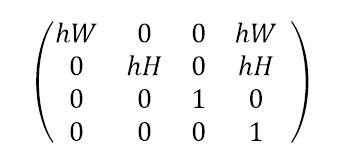
\includegraphics[scale=0.8]{screen_space}
		\caption[Матрица преобразования сцены в пространство изображения]{
			Матрица преобразования сцены в пространство изображения \par где:\\
			W -- ширина изображения, \\
			H -- высота изображения, \\
			hW -- половина ширины изображения,\\
			hH -- половина высоты изображения\\
		}
	\end{figure}

	\subsection{Выводы}
	 \quad Для получения итогового изображения на экране, необходимо применить ряд преобразований к объектам в сцене с ипользованием матриц.

	
	
	
	\section{Анализ алгоритмов закраски}
	\subsection{Однотонная закраска}
	 \quad В данном методе закраски цвет всей поверхности рассчитывается согласно закону Ламберта. Он формулируется так: плоская поверхность, имеющая одинаковую яркость по всем направлениям, отражает свет, интенсивность которого изменяется по закону косинуса --  $I = I_0  \cos \theta$, где $I_0$ -- интенсивность отражения в направлении нормали к поверхности, $\theta$ – угол между направлением на наблюдателя и нормалью к поверхности. 
	
	 Данный метод позволяет получать изображения, сравнимые по качеству с реальными объектами, лишь при выполнении следующих условий:
	\begin{enumerate}
		\item Источник света  и наблюдатель находятся на большом расстоянии от объекта.
		\item Каждая грань тела является гранью многогранника, а не аппроксимирующей поверхностью.
		\item Поверхность аппроксимирована большим числом небольших плоских граней.
	\end{enumerate}

	 Преимуществами этого метода закраски является простая реализация, а также небольшие требования к ресурсам. В то же время данный метод имеет ряд существенных недостатков. Так, например, он плохо подходит для гладких объектов и плохо учитывает отраженный свет, ярко выражает края фигур.
	
	\subsection{Метод закраски Гуро}
	 \quad Метод закраски Гуро основан на интерполяции интенсивности. Он позволяет устранить дискретность изменения интенсивности и создать иллюзию гладкой криволинейной поверхности.
	
	 Процесс закраски по методу Гуро осуществляется в четыре этапа:
	\begin{enumerate}
		\item Вычисляются нормали ко всем полигонам.
		\item Определяются нормали в вершинах путем усреднения нормалей по всем полигональным граням, которым принадлежит рассматриваемая вершина, как показано на рисунке 1.16.
		\item Используя нормали в вершинах, и применяя определенную модель освещения, вычисляют значения интенсивностей в вершинах многоугольника. 
		\item Каждый многоугольник закрашивается путем линейной интерполяции значений интенсивностей в вершинах сначала вдоль каждого ребра, а затем и между ребрами вдоль каждой сканирующей строки. 
	\end{enumerate}

	\begin{figure}[H]
		\centering
		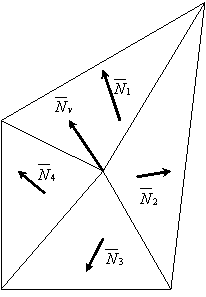
\includegraphics[scale=0.7]{normals}
		\caption{Определение нормалей}
	\end{figure}

	 Метод Гуро применим только для небольших граней, расположенных на значительном расстоянии от источника света. Если же размер грани достаточно велик, то расстояние от источника света до ее центра будет значительно меньше, чем до ее вершин, и, согласно закону освещенности, центр грани должен быть освещен сильнее ребер. Однако модель изменения освещенности, принятая в методе Гуро, предполагает линейное изменение яркости в пределах грани и не позволяет сделать середину грани ярче, чем ее края. В итоге на изображении появляются участки с неестественной освещенностью.
	
	\subsection{Метод закраски Фонга}
	 \quad Метод закраски Фонга основан на интерполяции вектора нормали, который затем используется в модели освещения для вычисления интенсивности пиксела.  
	
	 Процесс закраски по методу Фонга осуществляется в четыре этапа: 
	\begin{enumerate}
		\item Определяются нормали к граням.
		\item По нормалям к граням определяются нормали в вершинах.
		\item В каждой точке закрашиваемой грани определяется интерполированный вектор нормали.
		\item По направлению векторов нормали определяется цвет точек грани. 
	\end{enumerate}

	 Закраска Фонга требует больших вычислительных затрат, однако при этом достигается лучшая локальная аппроксимация кривизны поверхности, получается более реалистичное изображение, правдоподобнее выглядят зеркальные блики.
	
	\subsection{Выводы}
	 \quad Исходя из поставленной задачи, вместе с методом z-буфера предпочтительнее использовать алгоритм Гуро, сочетая приемлемую скорость работы и качество получаемого изображения.
		
	\section{Алгоритмы, моделирующие освещение}
	
	 \quad Реалистичность моделируемого изображения во многом зависит от правильного выбора модели освещения. В общем случае модели освещения делятся на локальные и глобальные. Локальные модели освещения учитывают только первичные источники света, не учитывая перенос света между поверхностями. В свою очередь глобальные модели освещения затрагивают такие аспекты, как преломление света, многократное отражение света, и т.п. 
	
	\subsection{Модель Ламберта}
	
	\quad Модель Ламберта (рисунок 1.17) моделирует идеальное диффузное освещение. Считается, что свет при попадании на поверхность рассеивается равномерно во все стороны. При расчете такого освещения учитывается только ориентация поверхности (нормаль N) и направление на источник света (вектор L).  
	
	\begin{figure}[h]
		\centering
		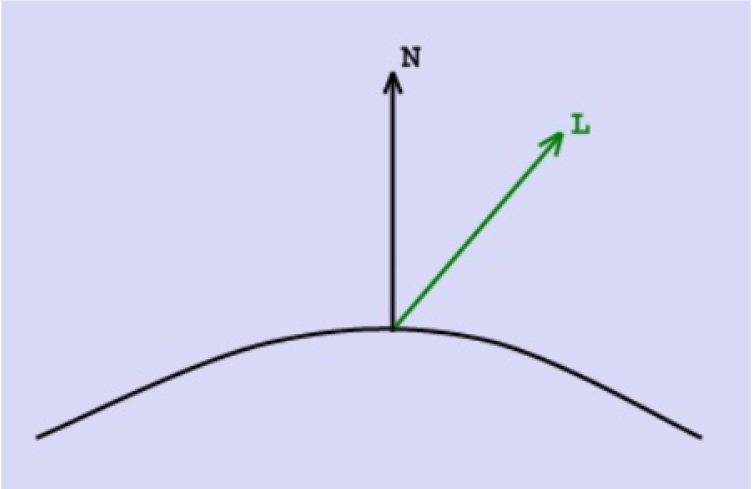
\includegraphics[width=0.7\linewidth]{lambert}
		\caption{Модель освещения Ламберта}
		\label{fig:screenshot001}
	\end{figure}

	Для удобства все векторы, описанные ниже, берутся единичными. В этом случае косинус угла между ними совпадает со скалярным произведением.
	%\Large
	\begin{equation}
		I_d = k_dcos(\vec L, \vec N)i_d=k_d(\vec L , \vec N)i_d
	\end{equation}
	

	 где:
	\begin{conditions*}
		I_d & рассеянная составляющая освещенности в точке,\\
		k_d  & свойство материала воспринимать рассеянное освещение,\\
		i_d  & интенсивность рассеянного освещения,\\
		L & направление на источник света,\\
		N & вектор нормали в точке
	\end{conditions*}
	
	 Модель Ламберта является одной из самых простых моделей освещения. Данная модель очень часто используется в комбинации других моделей, так как практически в любой модели освещения можно выделить диффузную составляющую. Более-менее равномерная часть освещения (без присутствия какого-либо всплеска) как правило будет представляться моделью Ламберта с определенными характеристиками. Данная модель может быть очень удобна для анализа свойств других моделей (за счет того, что ее легко выделить из любой модели и анализировать оставшиеся составляющие).
	
	
	\subsection{Модель Фонга}
	
	 \quad Основная идея модели Фонга заключается в предположении, что освещенность каждой точки тела разлагается на три компоненты:
	\begin{itemize}
		\item фоновое освещение (ambient);
		\item рассеянный свет (diffuse);
		\item бликовая составляющая (specular).
	\end{itemize}

	 Свойства источника определяют мощность излучения для каждой из этих компонент, а свойства материала поверхности определяют ее способность воспринимать каждый вид освещения.
	
	 Фоновое освещение присутствует в любом уголке сцены и никак не зависит от каких-либо источников света, поэтому для упрощения расчетов оно задается константой. Диффузное освещение рассчитывается аналогично модели Ламберта. Отраженная составляющая освещенности (блики) в точке зависит от того, насколько близки направления вектора, направленного на наблюдателя (вектор V на рисунке 1.18), и отраженного луча (вектор R на рисунке 1.18).
	
	 Падающий и отраженный лучи лежат в одной плоскости с нормалью к отражающей поверхности в точке падения, и эта нормаль делит угол между лучами на две равные части. Таким образом отраженная составляющая освещенности в точке зависит от того, насколько близки направления на наблюдателя и отраженного луча.
	
	\begin{figure}[h]
		\centering
		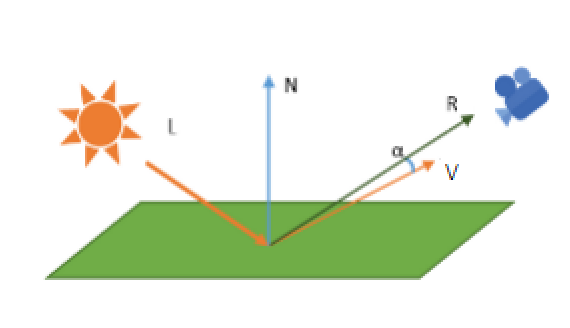
\includegraphics[width=0.7\linewidth]{ph}
		\caption{Получение бликов в модели освещения Фонга}
		\label{fig:screenshot003}
	\end{figure}

	 Интенсивность света в точке рассчитывается:
	\begin{equation}
	I_a = k_a I_a + k_d (\vec{N}, \vec{L}) + k_s (\vec{R}, \vec{V})^{p}
	\end{equation}
	где:
	\begin{conditions*}
		\vec{N} & вектор нормали к поверхности в точке,\\
		\vec{L} & падающий луч (направление на источник света),\\
		\vec{R} & отраженный луч,\\
		\vec{V} & вектор, направленный к наблюдателю,\\
		k_a & коэффициент фонового освещения,\\
		k_d & коэффициент диффузного освещения,\\
		k_s & коэффициент зеркального освещения,\\
		p & степень, аппроксимирующая пространственное распределение зеркально отраженного света.
	\end{conditions*}
	
	 Все векторы являются единичными. Модель Фонга улучшает визуальные качества сцены, по сравнению с моделью Ламберта, добавляя в нее блики (рисунок 1.19)
	
	\begin{figure}[h]
		\centering
		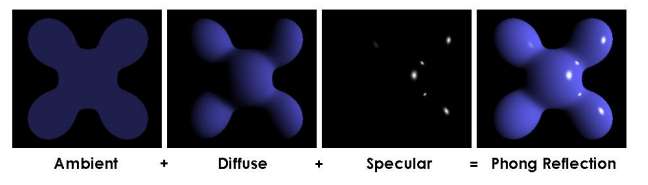
\includegraphics[width=0.7\linewidth]{ph_new}
		\caption{Модель освещения Фонга}
		\label{fig:screenshot003}
	\end{figure}
	
	\section{Вывод}
	 \quad В результате анализа алгоритмов, в соответствии с поставленной задачей для расчета интенсивности в точке была выбрана модель Ламберта при отрисовке сцены с использованием z-буфера и модель Фонга при использовании обратной трассировки лучей, так как  она позволяет учитывать матовые и блестящие поверхности, тем самым делая изображение более реалистичным.
	
	
	\chapter{Конструкторский раздел}
	 \quad После выбора алгоритмов, которые будут использоваться в курсовом проекте, составляется формальное описание выбранных алгоритмов в формате схем алгоритмов, а также приводятся математические выкладки.

	\newpage
	\section{Алгоритм удаления невидимых граней с использованием z-буфера}
	
	\quad На рисунке 2.1 приведена схема алгоритма z-буфера. 
	
	\begin{figure}[H]
		\centering
		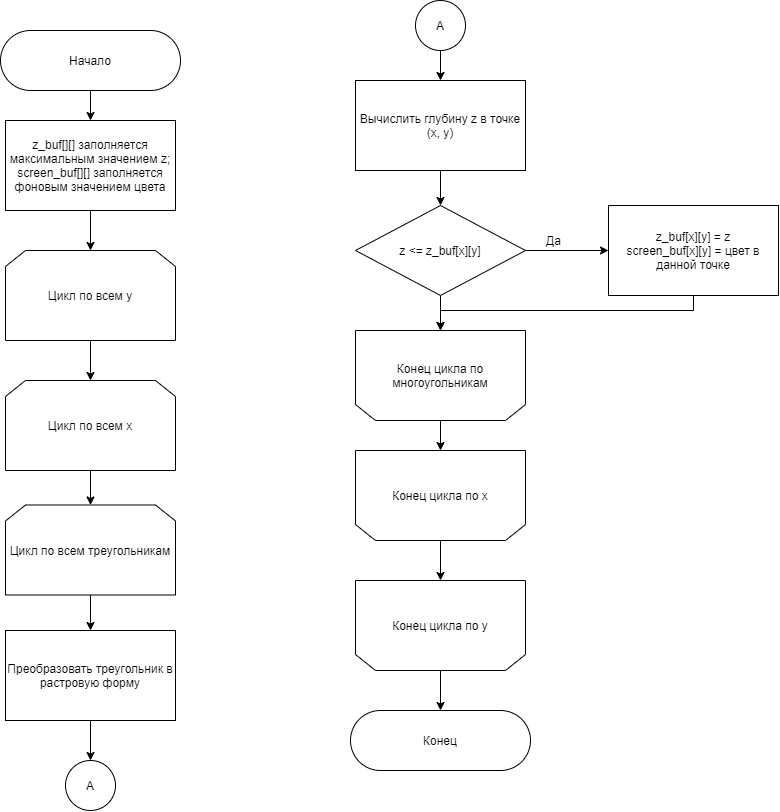
\includegraphics[scale=0.6]{z_buffer}
		\caption{Алгоритм z-буфера}
		\label{fig:z}
	\end{figure}

	\section{Алгоритм обратной трассировки лучей}
	
	\quad На рисунке 2.2 приведена схема алгоритма обратной трассировки лучей. 
	
	\begin{figure}[H]
		\centering
		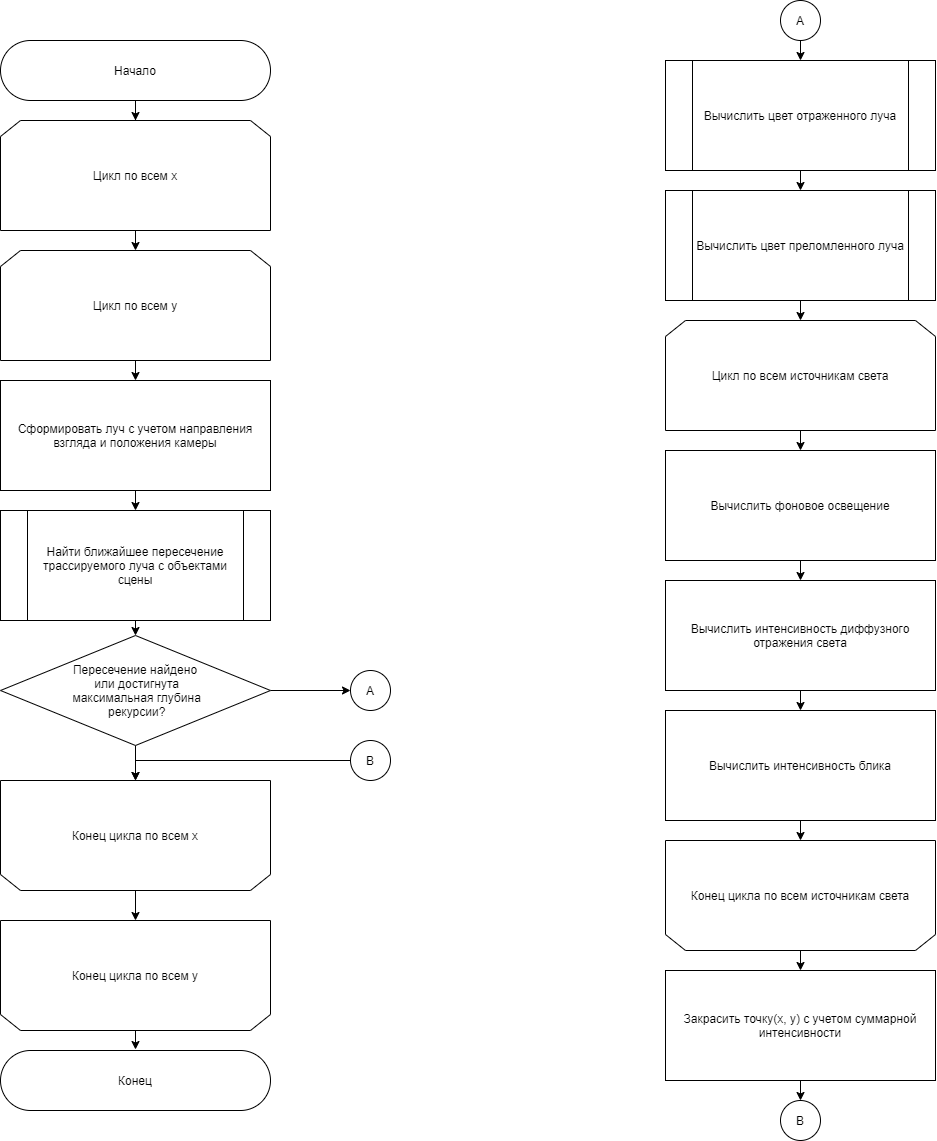
\includegraphics[scale=0.5]{trace}
		\caption{Алгоритм обратной трассировки лучей}
		\label{fig:z}
	\end{figure}

	\section{Пересечение трассирующего луча с треугольником}
	 \quad Для определения пересечения прямой (луча) и треугольника в трёхмерном пространстве удобно использовать алгоритм Моллера — Трумбора, для работы которого не требуется предварительное вычисление уравнения плоскости, содержащей треугольник.
	
	 Пусть точка на треугольнике $T(u, v)$ записана как:
	\begin{equation}
	T(u,v) = (1 - u - v) V_0 + u  V_1 + v  V_2
	\end{equation}
	где:
	\begin{conditions*}
		(u, v)     &  это барицентрические координаты, которые должны удовлетоврять условиям: $u \geqslant 0, v \geqslant 0$ и $ u + v \leqslant 1$. \\
	\end{conditions*}
	
	 Вычисление точки пересечения луча $R(t)$ и треугольника $T(u, v)$ эквивалентно решению уравнения $R(t) = T(u, v)$, которое записывается как:
	
	\begin{equation}
	O + tD = (1 - u - v) V_0 + u V_1 + v V_2
	\end{equation}
	где:
	\begin{conditions*}
		O & точка начала луча,\\
		D  & вектор направления луча,\\
		t  & любое вещественное число
	\end{conditions*}
	
	 Перегруппировав члены, получим:
	\def\C{
		\begin{bmatrix}
			t \\
			u \\
			v\\
	\end{bmatrix}}

	\begin{equation}
	\left[ -D, V_1 - V_0, V_2 - V_0\right] \C = O - V_0
	\end{equation}
	
	 Это значит, что барицентрические координаты $(u, v)$  и расстояние $t$  от начала луча до точки пересечения могут быть найдены из решения системы линейных уравнений выше.
	
	 Обозначим $E1 = V_1 - V_0$ , $E2 = V_2 - V_0$ и $T = O - V_0$. Проведя алгебраические преобразования можно получить формулу в следующем виде
	\def\D{
		\begin{bmatrix}
			dot(Q, E_2)\\
			dot(P, T)\\
			dot(Q, D)\\
	\end{bmatrix}}

	\begin{equation}
	\C = \frac{1}{dot(P, E_1)} \D
	\end{equation}
	где:
	
	\begin{conditions_eq*}
		P & $(D \times E_2)$ ,\\
		Q & $(T \times E_1)$
	\end{conditions_eq*}

	\section{Алгоритм нахождения пересечения луча с параллелепипедом}
	 \quad При работе алгоритма обратной трассировки лучей крайне неэффективно при каждой трассировке луча искать пересечения со всеми полигонами каждого объекта в сцене, поэтому имеет смысл заключить каждый объект в параллелипипед, который бы полностью его включал.
	
	 Данный параллелепипед задается координатами двух вершин: с минимальными и максимальными значениями координат x, y, z. Таким образом это позволяет задать шесть плоскостей, ограничивающих параллелепипед, и при этом  все они будут параллельны координатным плоскостям (рисунок 2.3).
	
	\begin{figure}[h]
		\centering
		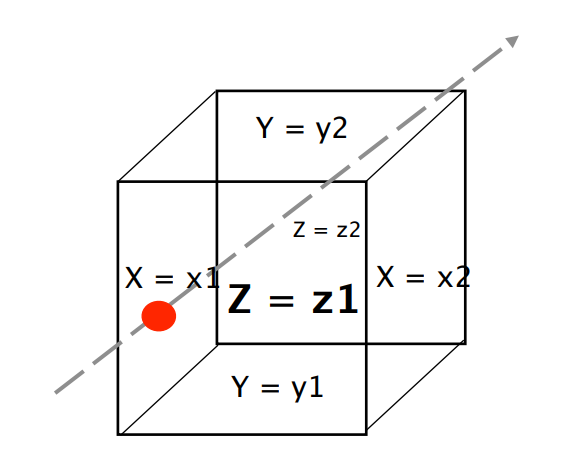
\includegraphics[scale=0.7]{cube}
		\caption{Пересечение луча с параллелепипедом}
	\end{figure}

	 Рассмотрим пару плоскостей, параллельных плоскости yz: X = $x_1$ и X = $x_2$. Пусть $\vec{D}$ –- вектор направления луча. Если координата х вектора $\vec{D}$ равна 0, то заданный луч параллелен этим плоскостям и, если $x_0 < x_1$ или $x_0 > x_1$, то он не пересекает рассматриваемый прямоугольный параллелепипед. Если же Dx не равно 0, то вычисляются отношения:
	\begin{equation}
	\begin{gathered}
		t1x = \frac{(x_1 - x_0)}{Dx}\\
		t2x = \frac{(x_2 - x_0)}{Dx}
	\end{gathered}
	\end{equation}
	
	 Можно считать, что найденные величины связаны неравенством t1x < t2x.
	
	 Пусть tn = t1x, tf = t2x. Считая, что Dy не равно 0, и рассматривая вторую пару плоскостей, несущих грани заданного параллелепипеда, $Y = y_1$ и $Y = y_2$, вычисляются величины:
	
	\begin{equation}
	\begin{gathered}
	t1y = \frac{(y_1 - y_0)}{Dy}\\
	t2y = \frac{(y_2 - y_0)}{Dy}
	\end{gathered}
	\end{equation}
	
	 Если t1y > tn, тогда пусть tn = t1y. Если t2y < tf, тогда пусть tf = t2y.
	При tn > tf или при tf < 0 заданный луч проходит мимо прямоугольного параллелепипеда.
	
	 Считая, что Dz не равно 0, и рассматривая вторую пару плоскостей, несущих грани заданного параллелепипеда, $Z = z_1$ и $Z = z_2$, вычисляются величины:
	
	\begin{equation}
	\begin{gathered}
	t1z = \frac{(z_1 - z_0)}{Dz}\\
	t2z = \frac{(z_2 - z_0)}{Dz}
	\end{gathered}
	\end{equation}
	и повторяются сравнения описанные выше.
	
	 Если в итоге всех проведенных операций получается, что 0 < tn < tf или 0 < tf, то заданный луч пересечет исходный параллелепипед со сторонами, параллельными координатным осям.
	
	 Следует отметить, что при пересечении лучом параллелепипеда извне знаки tn и tf должны быть равны, в противном случае можно сделать вывод, что луч пересекает параллелепипед изнутри.
	
	\section{Нахождение отраженного луча}
	
	 \quad Для нахождения направления отраженного луча достаточно знать направление падающего луча $\vec{L}$ и нормаль к поверхности $\vec{N}$ в точке падения луча.
	
	 Можно разложить $\vec{L}$ на два вектора $\vec{L_p}$ и $\vec{L_n}$, таких что $\vec{L} = \vec{L_p} + \vec{L_n}$, где $\vec{L_n}$ параллелен $\vec{N}$, а $\vec{L_p}$ перпендикулярен, как изображено на рисунке 2.4.
	
	
	\begin{figure}[h]
		\centering
		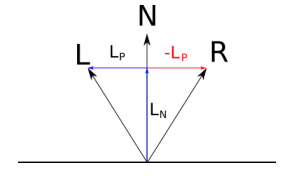
\includegraphics{reflect}
		\caption{Разложение вектора падающего луча}
	\end{figure}

    $\vec{L_n}$ -- проекция $\vec{L}$ на $\vec{N}$. По свойствам скалярного произведения и исходя из того, что $\abs{N} = 1$, длина этой проекции равна $(\vec{N},\vec{L})$, поэтому:
    \begin{equation}
    \vec{L_n} = \vec{N}(\vec{N}, \vec{L})
    \end{equation}
    
     Отсюда
    \begin{equation}
    \vec{L_p} = \vec{L} - \vec{L_n} = \vec{L} - \vec{N}(\vec{N}, \vec{L})
    \end{equation}
    
     Очевидно, что:
    \begin{equation}
    \vec{R} = \vec{L_n} - \vec{L_p}
    \end{equation}
    
     Подставив полученные ранее выражения и упростив, можно получить формулу отраженного луча:
    \begin{equation}
    \vec{R} = 2\vec{N}(\vec{N}, \vec{L}) - \vec{L}
    \end{equation}
    
    \section{Расчет интенсивностей}
     \quad Интенсивность света, диффузно отражающегося в точке поверхности, можно вычислить следующим образом (не зависит от положения наблюдателя):
    
    \begin{equation}
    I_d = k_d  \sum_{i=1}^{n}I  (\vec{N}, \vec{L_i})
    \end{equation}
    где:
    \begin{conditions*}
    	k_d & коэффициент диффузного отражения,\\
    	I_i  & интенсивность света, попадающего в точку от i-го источника освещения,\\
    	\vec{N}  & нормаль к поверхности в данной точке,\\
    	\vec{L_i} & единичный вектор, совпадающий по направлению с вектором, проведенным из i-го источника в рассматриваемую точку,\\
    	n & количество всех источников в сцене
    \end{conditions*}

	 Интенсивность света, отраженного зеркально, может быть вычислена следующим образом (зависит от положения наблюдателя):
	
	\begin{equation}
	I_s = k_s  \sum_{i=1}^{n}I  (\vec{S}, \vec{R_i})^{n_p}
	\end{equation}
	где:
	\begin{conditions*}
		k_s & коэффициент зеркального отражения,\\
		I_i  & интенсивность света, попадающего в точку от i-го источника освещения,\\
		\vec{S}  & единичный вектор, совпадающий по направлению с вектором из рассматриваемой точки в точку наблюдения,\\
		\vec{R_i} & единичный вектор, задающий направление отраженного луча от i-го источника,\\
		n & количество всех источников в сцене,\\
		n_p & степень, аппроксимирующая пространственное распределение зеркально отраженного света
	\end{conditions*}

	 Общую интенсивность можно определить по формуле:
	\begin{equation}
	I_r = k_a  \sum_{i=1}^{n}I_ia + k_d  \sum_{i=1}^{n}I  (\vec{N}, \vec{L_i}) +  k_s  \sum_{i=1}^{n}I  (\vec{S}, \vec{R_i}^{n_p}) + k_r I_r + k_t I_t
	\end{equation}
	где:
	\begin{conditions*}
		k_s & коэффициент рассеянного отражения,\\
	    k_a & коэффициент зеркального отражения,\\
		k_d & коэффициент диффузного отражения,\\
		k_r & коэффициент отражения,\\
		k_t & коэффициент преломления,\\
		I_r, I_t  & интенсивности, принесенные составляющими оттрассированных отраженного и преломленного лучей,\\
		I_a & составляющие рассеянного освещения от i-го источника,\\
		\vec{S}  & единичный вектор, совпадающий по направлению с вектором из рассматриваемой точки в точку наблюдения,\\
		\vec{R_i} & единичный вектор, задающий направление отраженного луча от i-го источника,\\
		n & количество всех источников в сцене,\\
		N & степень, аппроксимирующая пространственное распределение зеркально отраженного света
	\end{conditions*}

	\section{Описание входных данных}
	 \quad В данной программе входные данные подаются в виде файла с расширением .obj. В этом формате помимо координат вершин можно передавать информацию о текстурах и нормалях. 	
	
	 Формат файла:
	
	\begin{enumerate}
		\item Список вершин с координатами (x,y,z).
		$$ \text{v 0.74 0.26 1} $$
		\item Текстурные координаты (u,v).
		$$ \text{vt 0.830 0.5} $$
		\item Координаты нормалей (x,y,z).
		$$ \text{vn 0.7 0.000 0.3} $$
		\item Определение поверхности (сторон) задается в формате i1/i2/i3, где i1 - индекс координаты вершины, i2 - индекс координаты текстуры, i3 - индекс координаты нормали.
		$$ \text{f 2/4/4 3/5/5 1/3/5} $$
	\end{enumerate}
		
	\chapter{Технологический раздел}
	 \quad Необходимо произвести выбор средств разработки программы, так как от выбора языка программирования зависит дальнейшая поддержка и возможности развития разработанного программного обеспечения. Помимо этого описать структуру программы, взаимодействие пользователя с графическим интерфейсом, представить листинги функций, описание которых потребуется в исследовательской части.
	
	\subsection{Средства реализации}
	 \quad Для решения поставленных в курсовом проекте задач был выбран язык программирования C++, поскольку:
	\begin{itemize}
		\item данный язык освоен ранее на практических занятиях;
		\item основной парадигмой в данном языке является ООП, что позволит разбить компоненты сцены на соответствующие классы; 
		\item C++ достаточно производительный, это будет большим плюсом при решении такой трудозатратной задачи, как трассировка лучей. 
	\end{itemize}

	 В качестве IDE был выбран “QT Creator” по следующим причинам: 
	
	\begin{itemize}
		\item знаком с данной IDE, т.к. делал в ней лабораторные работы по курсу «Компьютерная графика»;
		\item позволяет очень быстро создавать графические интерфейсы любой сложности.
	\end{itemize}

	\section{Описание структуры программы}
	 \quad В программе реализованы следующие классы:
	\begin{itemize}
		\item class Manager - описывает сцену и методы работы с ней;
		\item class Model - описывает способ хранения объекта и методы работы с ним;
		\item class Light - описывает атрибуты источников света различного света и содержит функции для работы со светом;
		\item class PixelShader - содержит функции для вычисления атрибутов объекта в конкретном пикселе;
		\item class VertexShader - содержит функции для преобразования атрибутов модели при переходе к мировому пространству из объектного;
		\item class TextureShader - содержит функции для интерполяции значения текстурных координат в конкретном пикселе;
		\item class GeometryShader - содержит функции для перехода из мирового пространства в пространство нормализованных координат;
		\item class Face - описывает полигон-треугольник;
		\item class Vertex - сожердит информацию о вершине полигона;
		\item class Vec3, class Vec4 - описывают вектора размерности 3 и 4, содержат функции для работы с ними;
		\item class Mat -  описывает матрицы произвольного размера и содержит функции для работы с ними;
		\item class Camera - описывает камеру;
		\item class BoundingBox - описывает параллельный осям ограничивающий параллелепипед и содержит функции для работы с ним;
		\item class RayThread - содержит функции для выполнения трассировки.
	\end{itemize}

	\section{Листинг кода}
	 \quad На листинге 3.1 представлена функция, отрисовывающая модель.
	
	\lstinputlisting[language=C++, caption = Функция отрисовки модели]{rasterize.txt}
	
	 На листинге 3.2 представлена функция растеризации треугольника.
	
	\lstinputlisting[language=C++, caption = Функция растеризации треугольника]{rasterTriangle.txt}
	
	 На листинге 3.3 представлена функция нахождения пересечения с ограничивающим параллелепипедом.
	
	\lstinputlisting[language=C++, caption = Функция нахождения пересечения с ограничивающим параллелепипедом]{aabb.txt}
	
	 На листинге 3.4 представлена оптимизация предыдущей функции.
	
	\lstinputlisting[language=C++, caption = Оптимизированная функция нахождения пересечения с ограничивающим параллелепипедом]{optimizedAA.txt}
	

	\section{Описание интерфейса}
	\quad  На рисунке 3.1 представлен интерфейс программы. 
	Он предусматривает возможность вращения, перемещения, масштабирования объектов, изменения свойств, цвета, текстуры их поверхности; добавления и удаления моделей и источников света, изменение параметров источников. Для обзора сцены используется камера, управление которой осуществляется посредством нажатия клавиш на клавиатуре.	
	
	\begin{figure}[H]
		\centering
		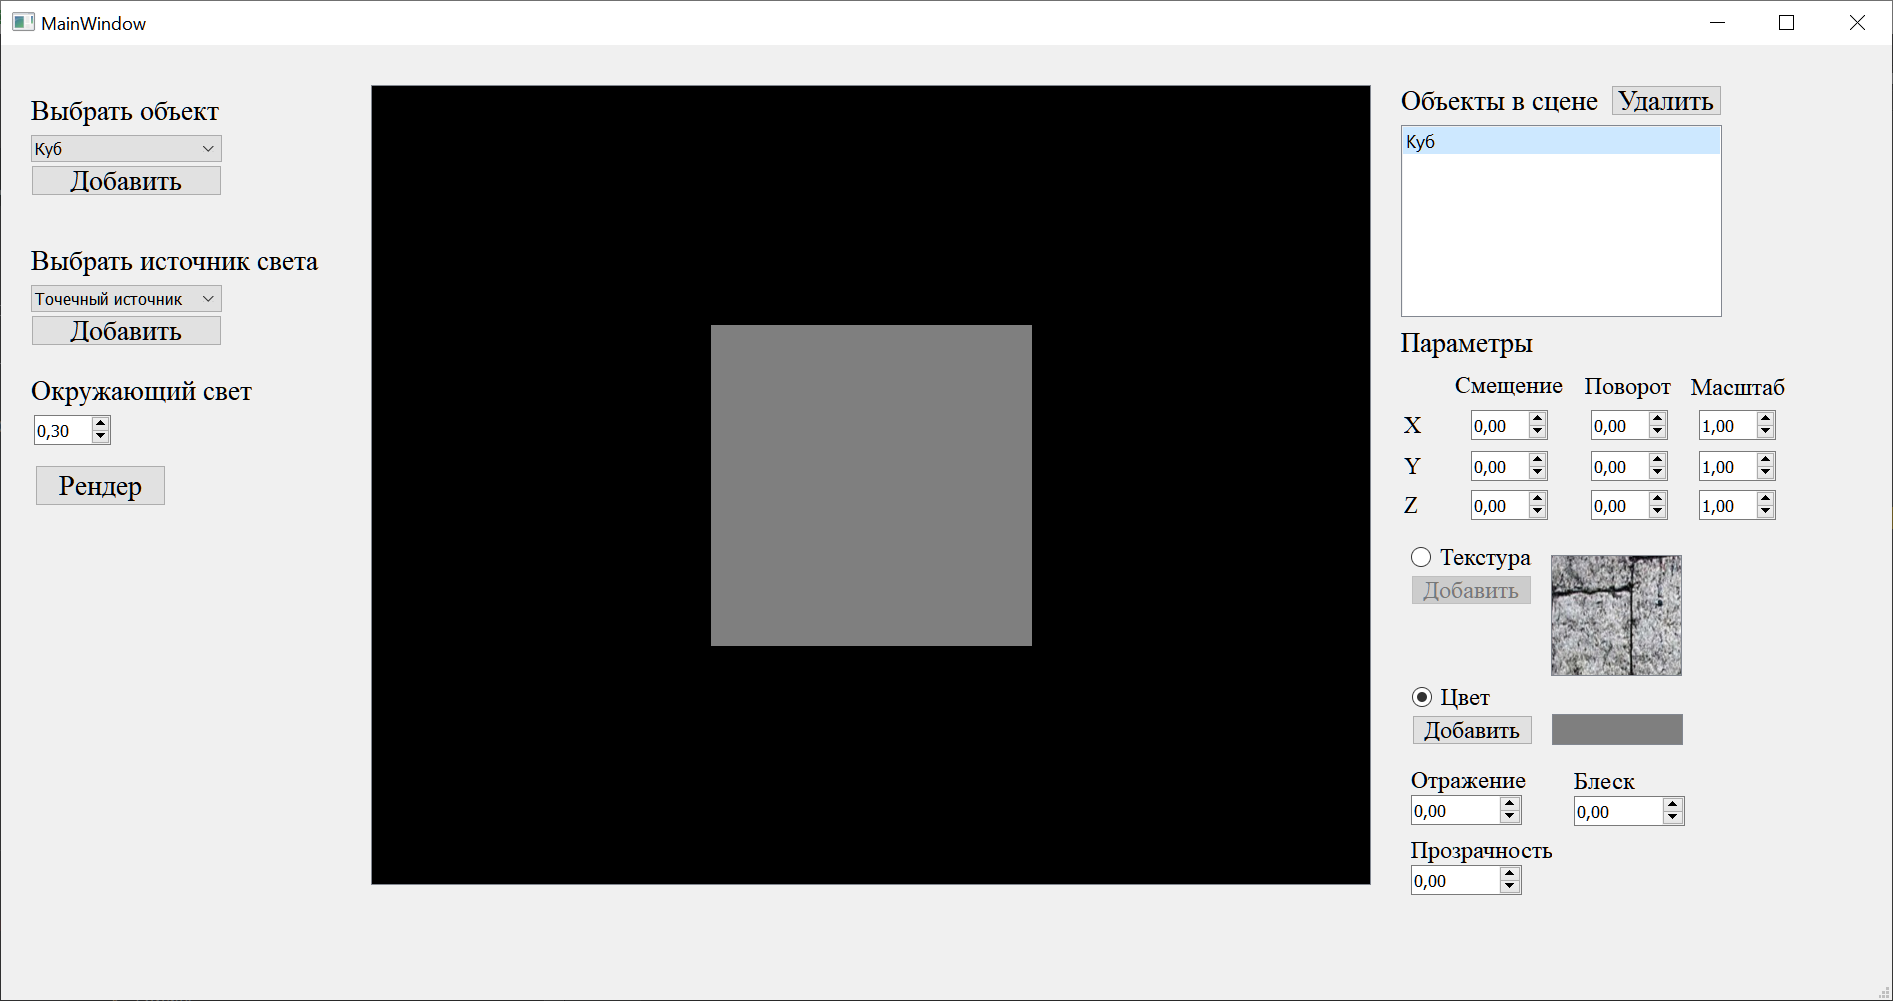
\includegraphics[scale = 0.5]{interface}
		\caption{Интерфейс программы}
	\end{figure}

	Для добавления модели на сцену нужно выбрать ее из списка (рисунок 3.2) и нажать на кнопку "добавить" под ним, после чего она будет отрисована на экране и попадет в список объектов в сцене в правом углу (рисунок 3.3). 
	
	 \begin{figure}[H]
		\centering
		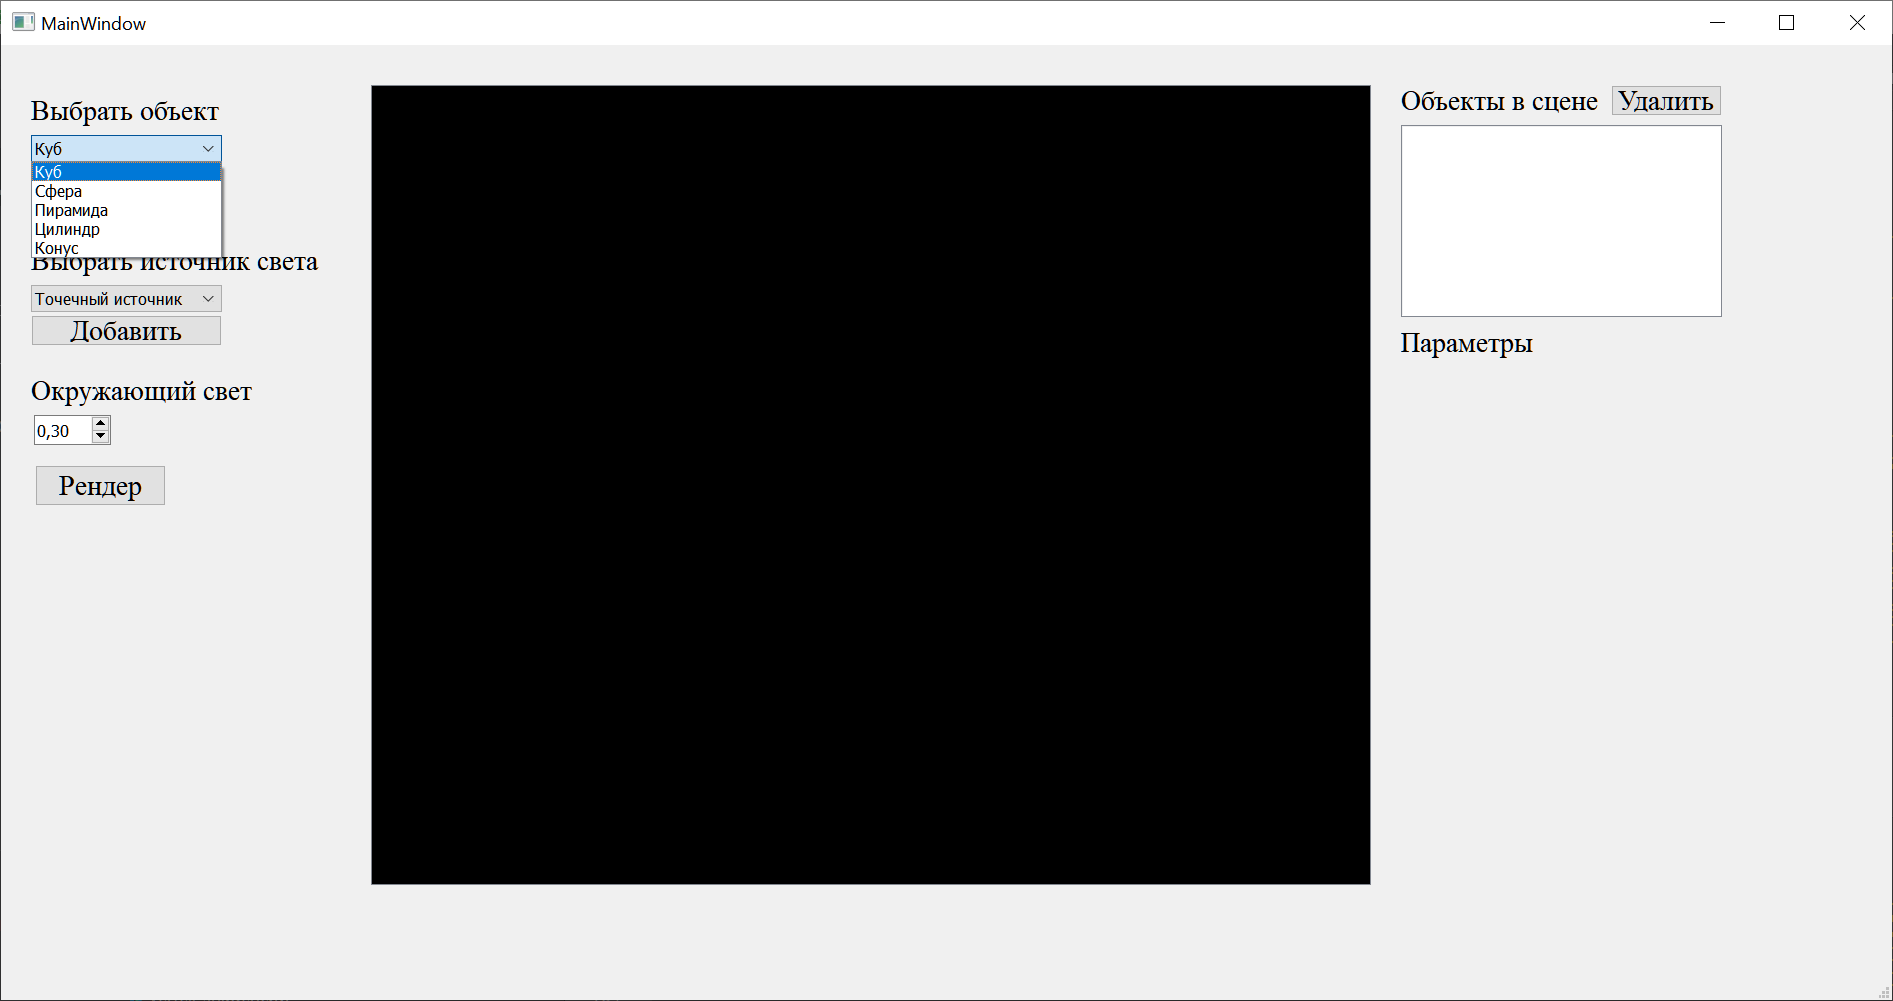
\includegraphics[scale = 0.5]{list}
		\caption{Список моделей для добавления}
	\end{figure}
	
	\begin{figure}[H]
		\centering
		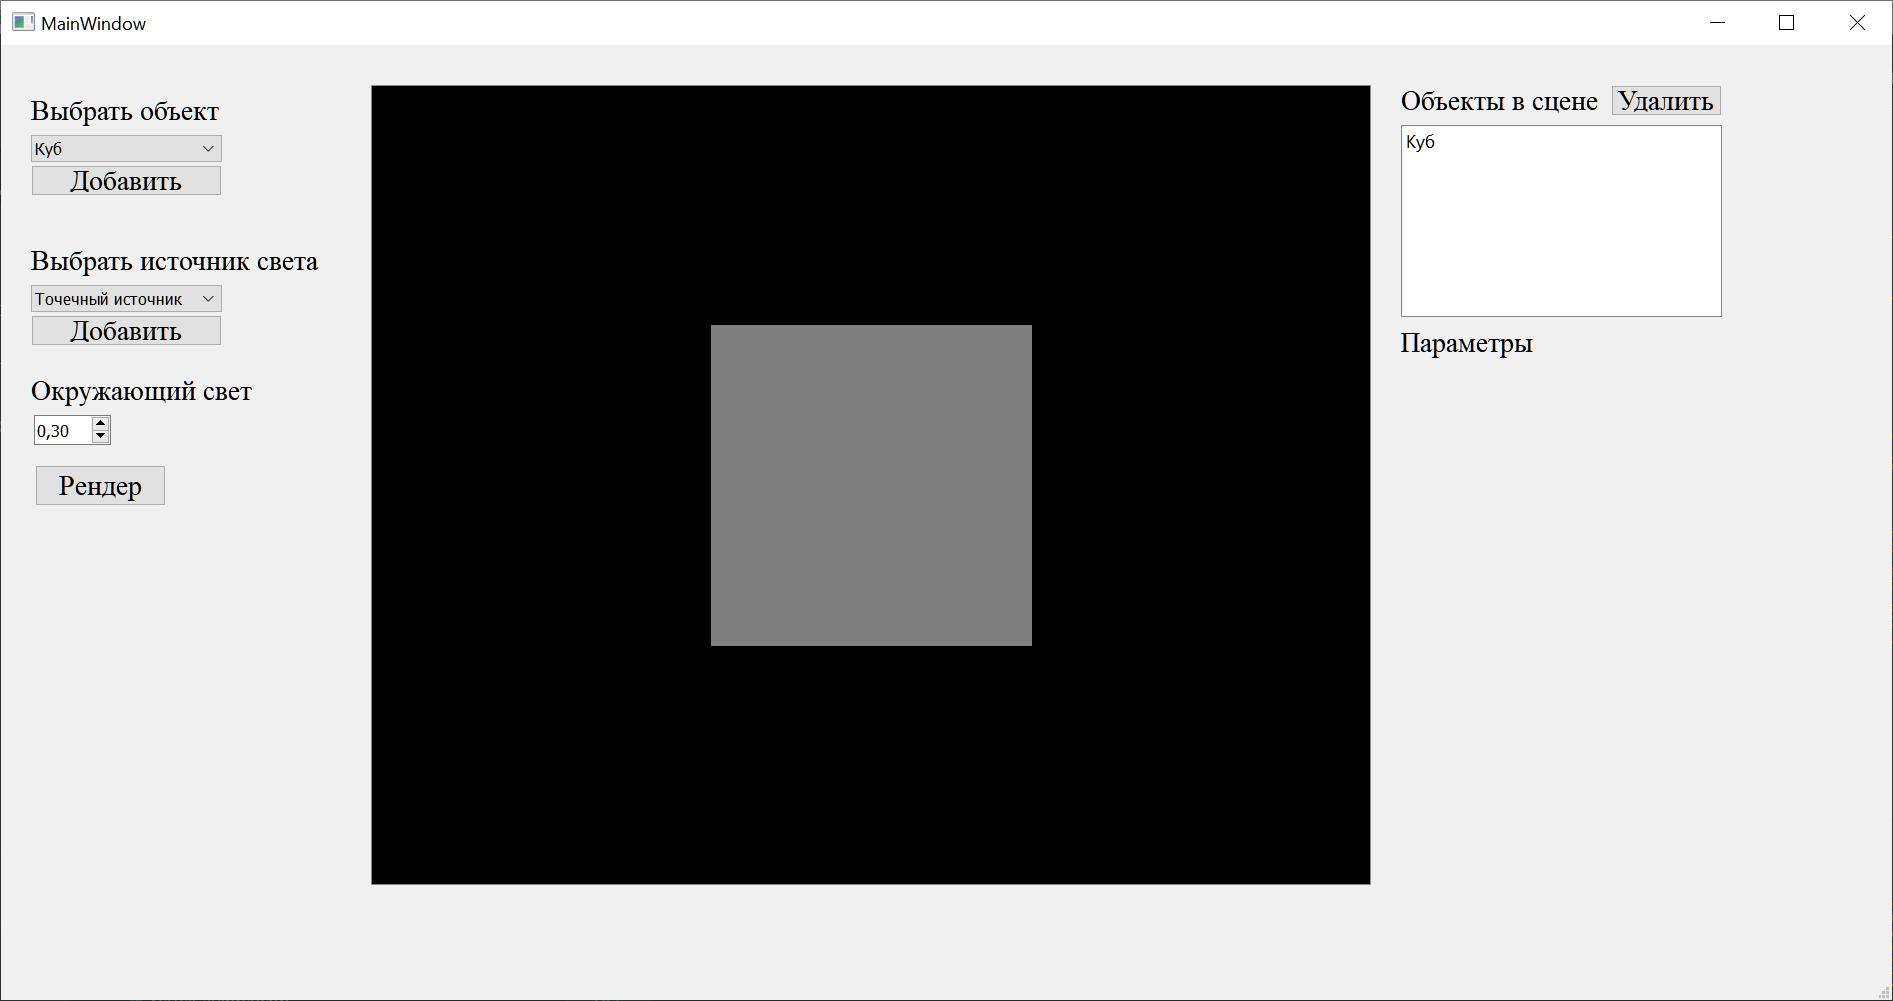
\includegraphics[scale = 0.5]{list_object}
		\caption{Список объектов в сцене в правом верхнем углу}
	\end{figure}

	Для изменения параметров модели нужно выбрать его из списка объектов в сцене, который находится в правом верхнем углу. После нажатия на название модели, в правой части экрана появится список параметров, доступных для изменения (рисунок 3.4). Изменение цвета и текстуры объекта происходит путем взаимодействия с диалоговыми окнами как показано на рисунке 3.5 и 3.6, которые открываются при нажати на соответствующие кнопки "Добавить". Для переключения между цветом и текстурой используются элементы RadioButton (рисунок 3.4).
	
	\begin{figure}[H]
		\centering
		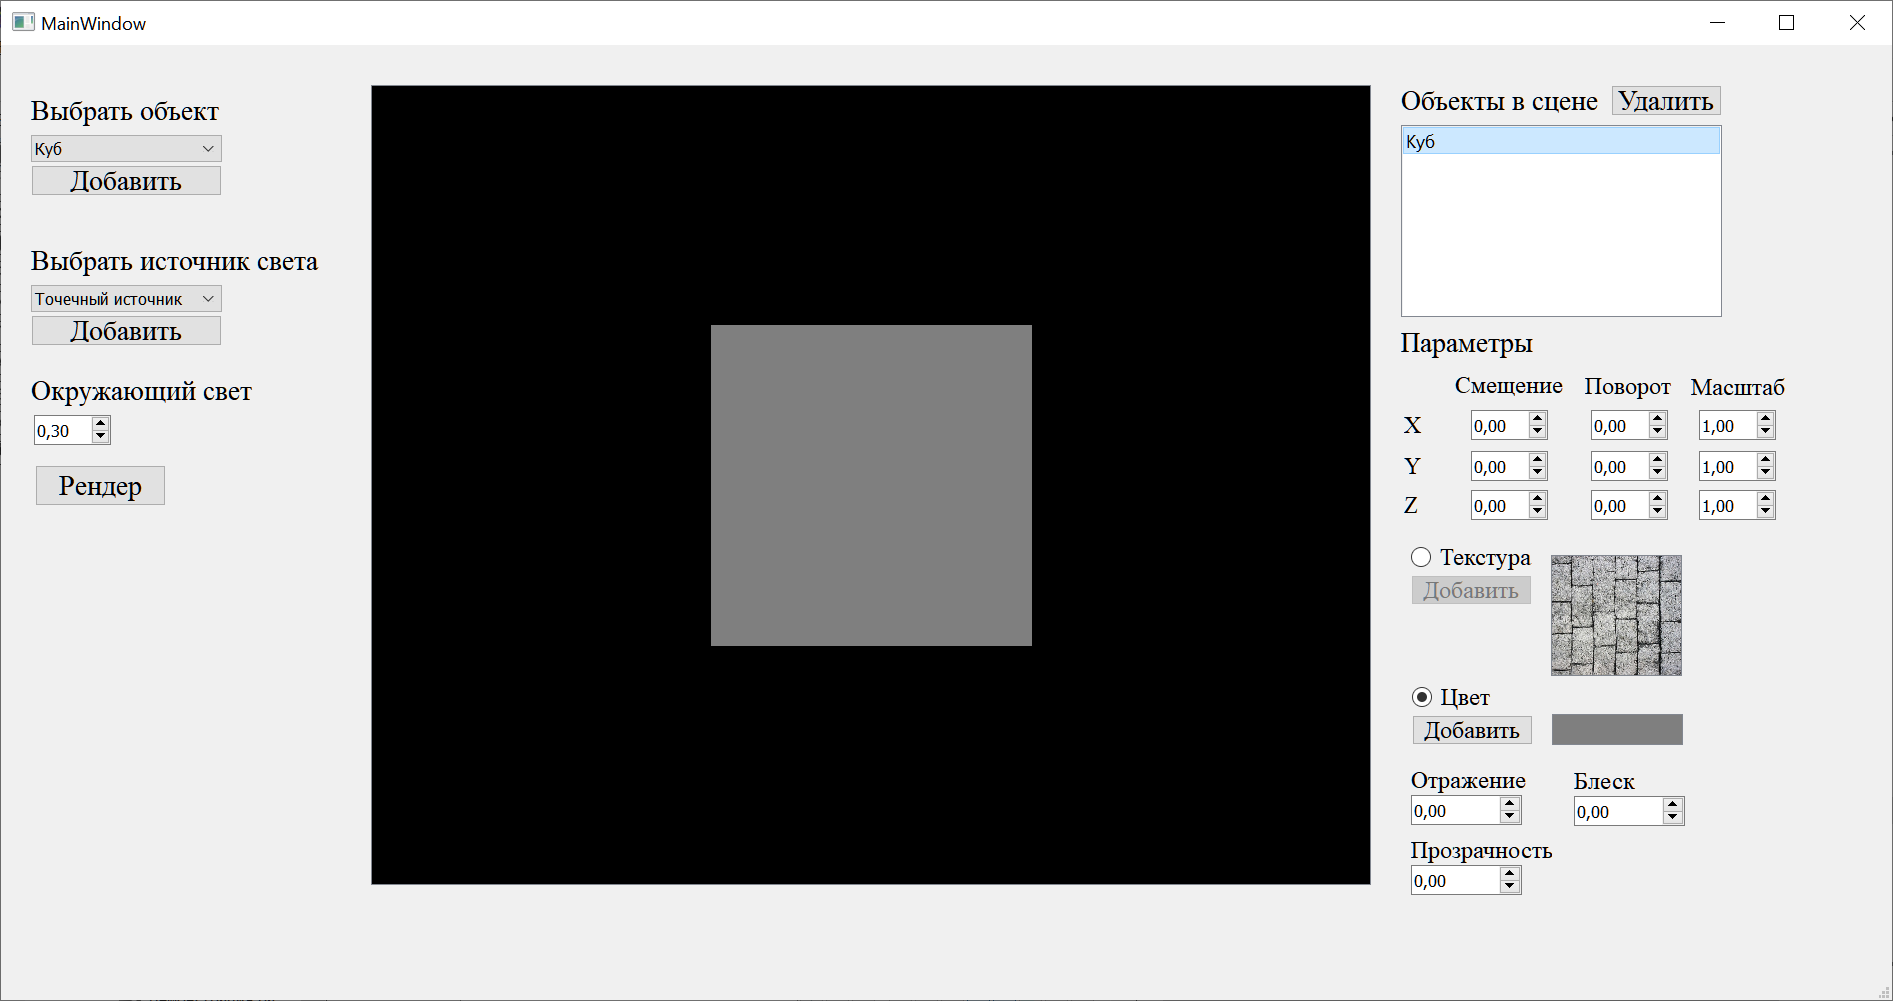
\includegraphics[scale = 0.5]{list_params}
		\caption{Список параметров модели}
	\end{figure}

	\begin{figure}[H]
		\centering
		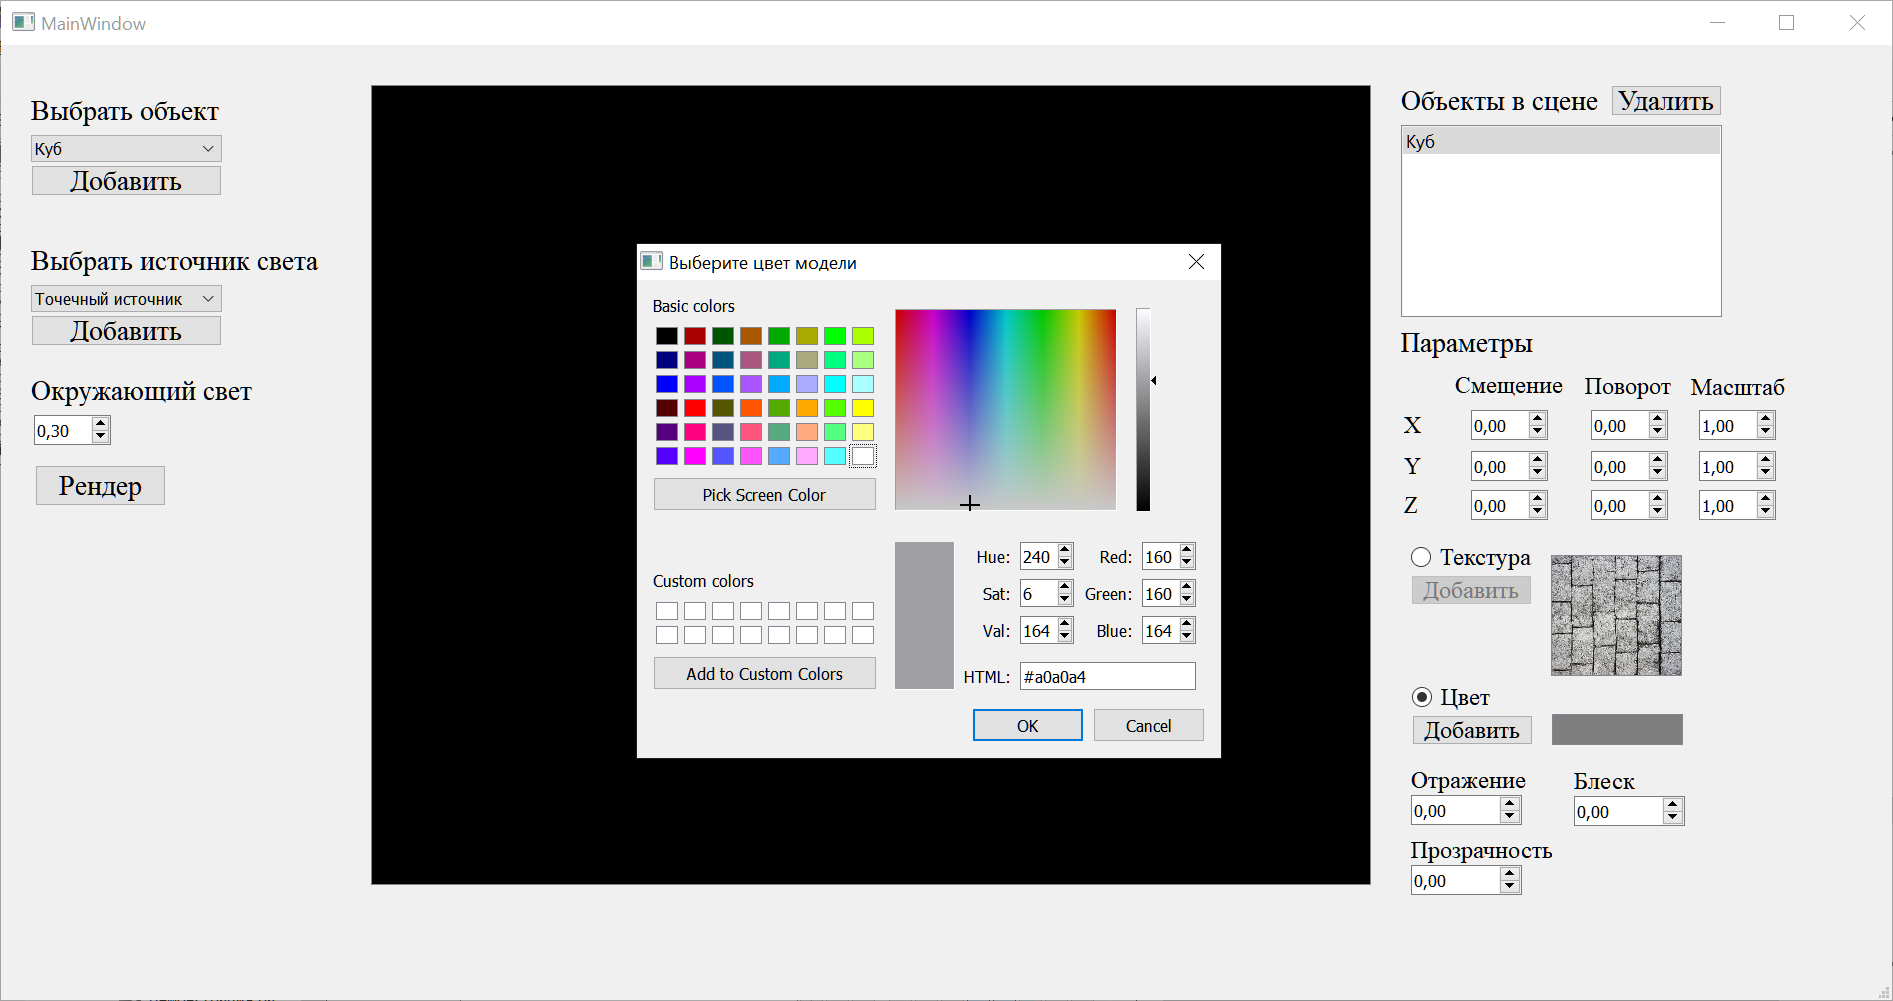
\includegraphics[scale = 0.5]{color_dialog}
		\caption{Диалоговое окно для выбора цвета}
	\end{figure}

	\begin{figure}[H]
		\centering
		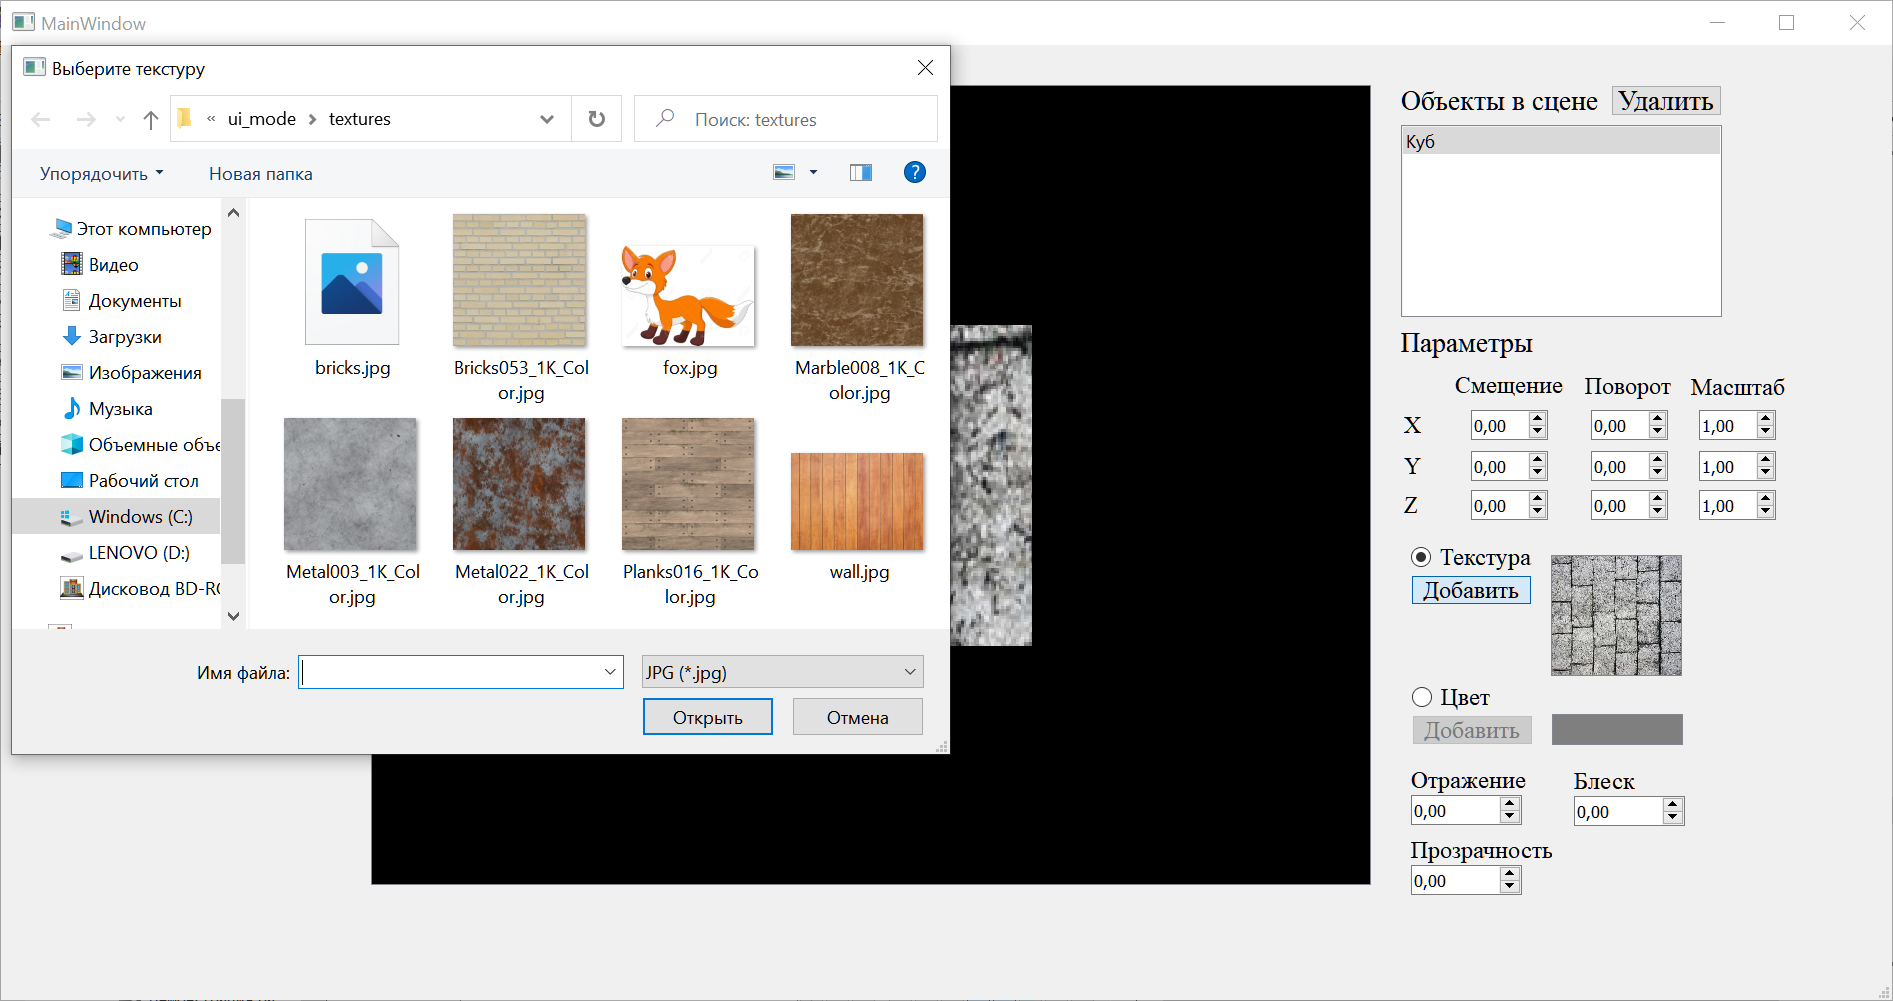
\includegraphics[scale = 0.5]{texture_dialog}
		\caption{Диалоговое окно для выбора текстуры}
	\end{figure}

	Источники света также выбираются из списка (рисунок 3.7) и при нажатии на кнопку "добавить" добавляются в список объектов, расположенный в правом верхнем углу, и отрисовываются на сцене. Точечный источник имеет форму сферы, а направленный форму "пули" (рисунок 3.8). При нажатии на источник в правой части появляется меню изменения его параметров(рисунок 3.8). Интенсивность окружающего освещения меняется в левой части экрана посредством взаимодействия с SpinBox.
	
	\begin{figure}[H]
		\centering
		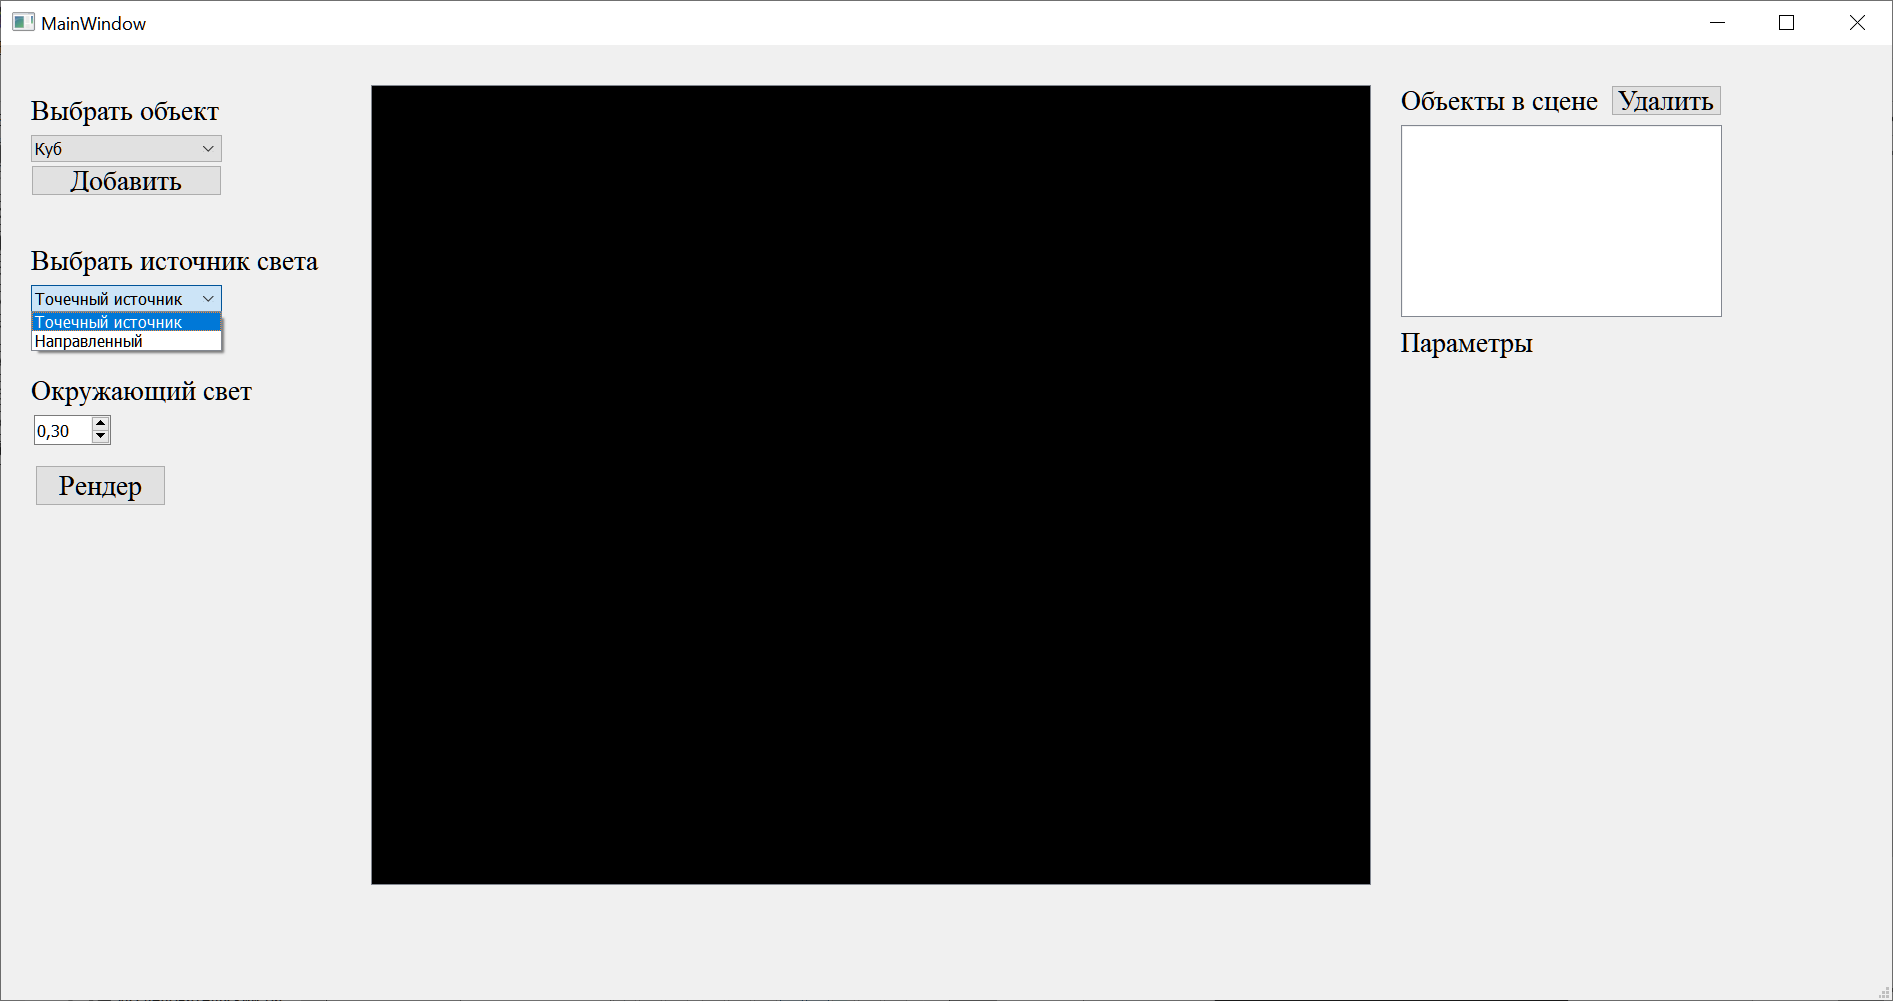
\includegraphics[scale = 0.5]{light_list}
		\caption{Список источников света}
	\end{figure}

	\begin{figure}[H]
		\centering
		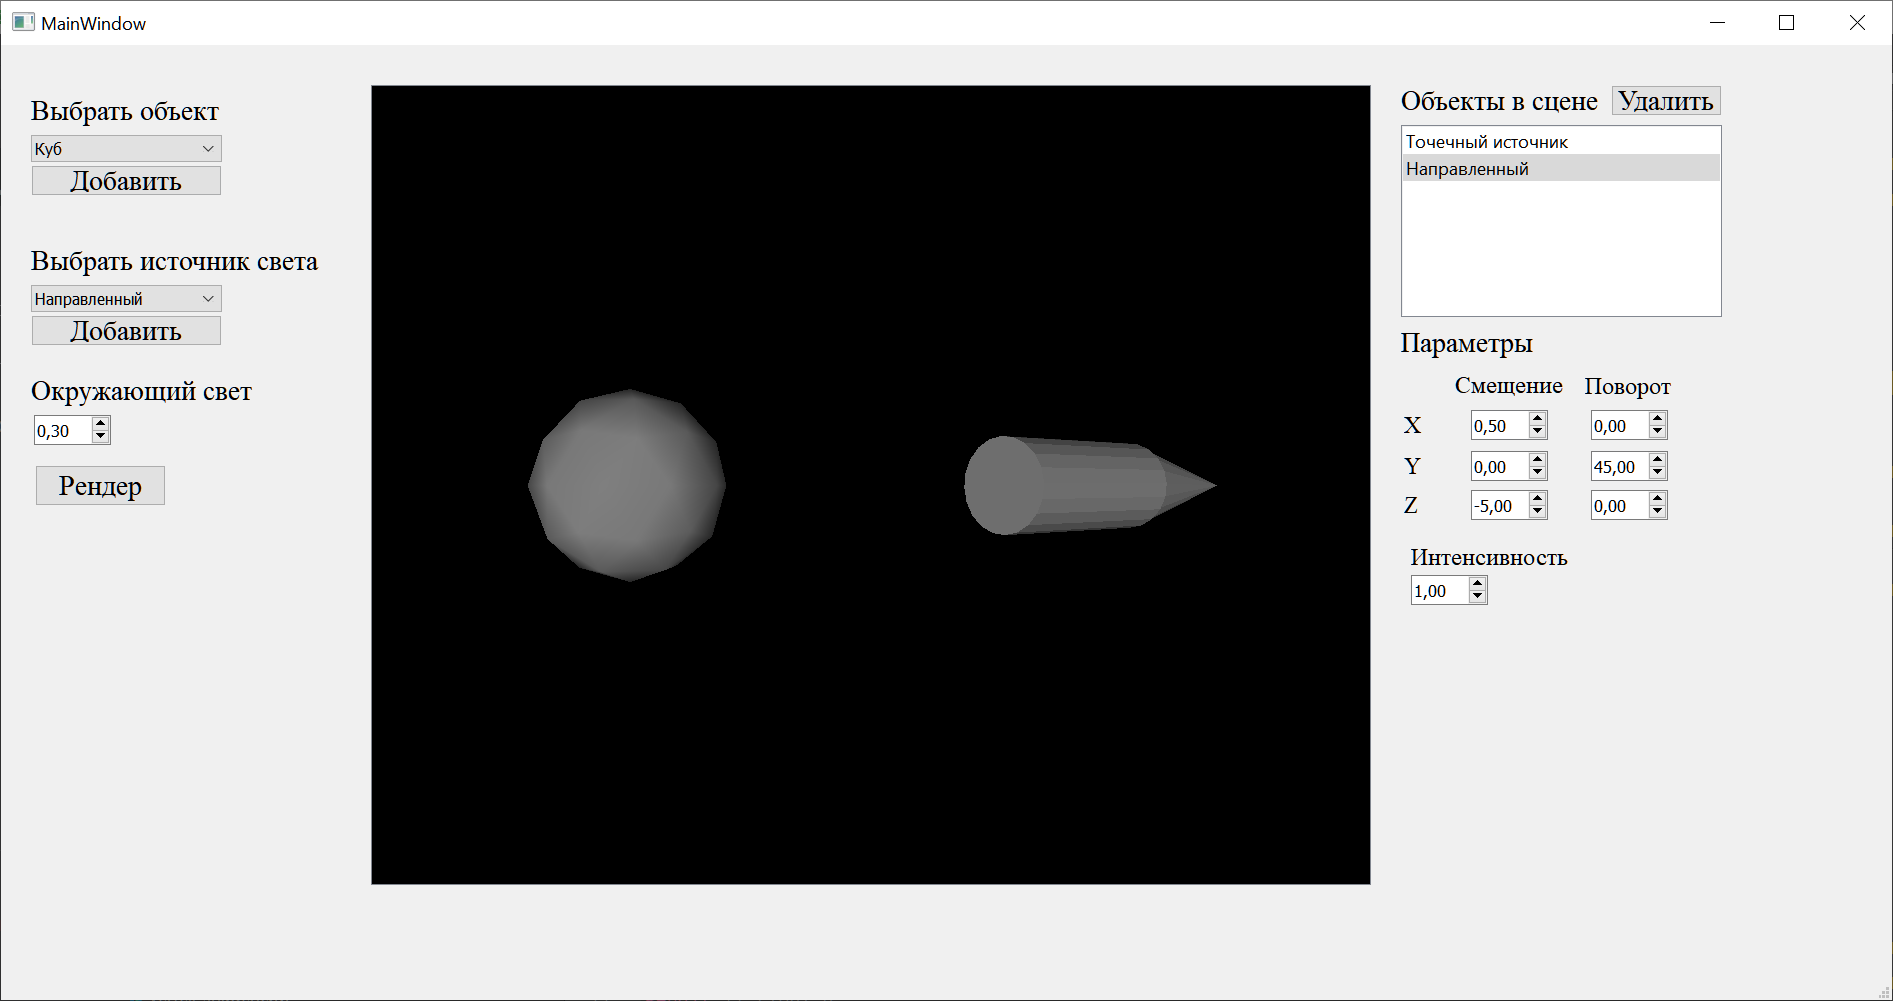
\includegraphics[scale = 0.5]{dir_point}
		\caption{Вид источников света в сцене}
	\end{figure}

	После добавления объектов и источников в сцену, задания необходимых параметров и выбора положения обзора, нажатие на кнопку "Рендер" запустит процесс генерации изображения с применением алгоритма обратной трассировки лучей, интерфейс будет заблокирован пока изображение не будет готово (рисунок 3.9). После получения результата (рисунок 3.10), к предыдущему режиму можно вернуться, нажав на кнопку "Рендер".

	\begin{figure}[h]
		\centering
		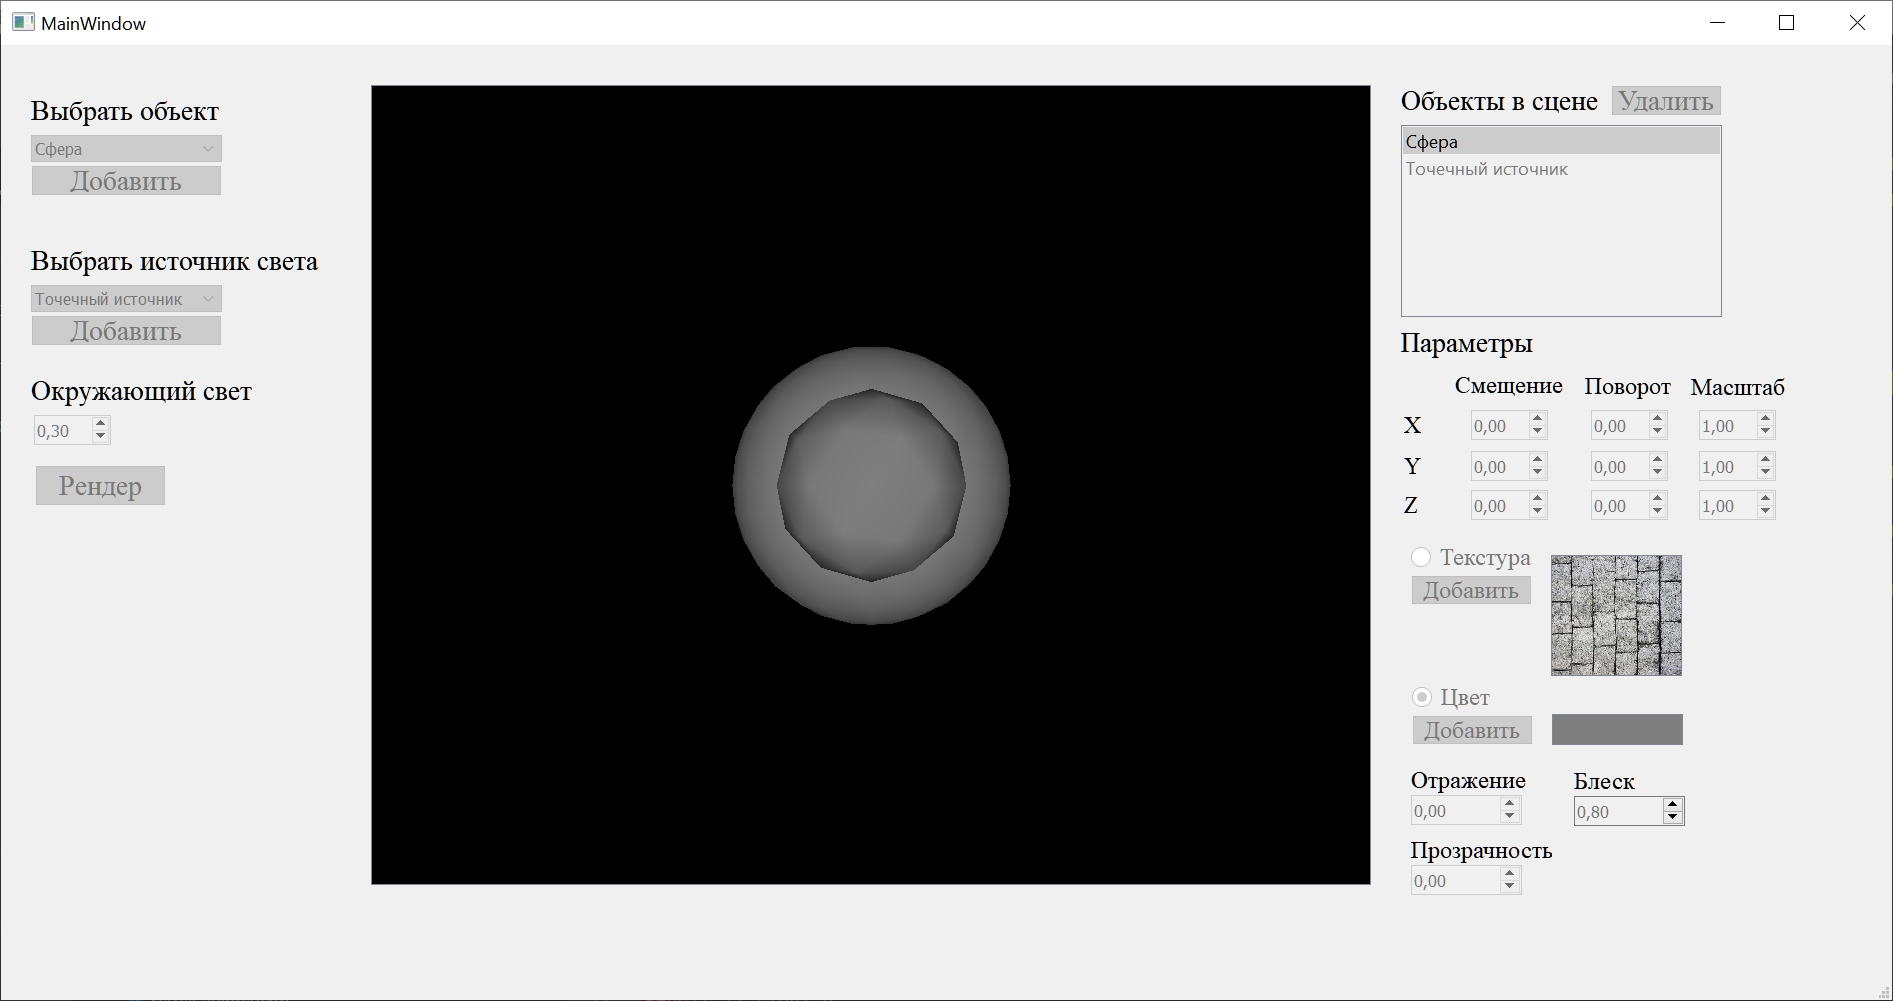
\includegraphics[scale = 0.5]{wait}
		\caption{Блокировка интерфейса в процессе выполнения рендеринга}
	\end{figure}

	\begin{figure}[h]
		\centering
		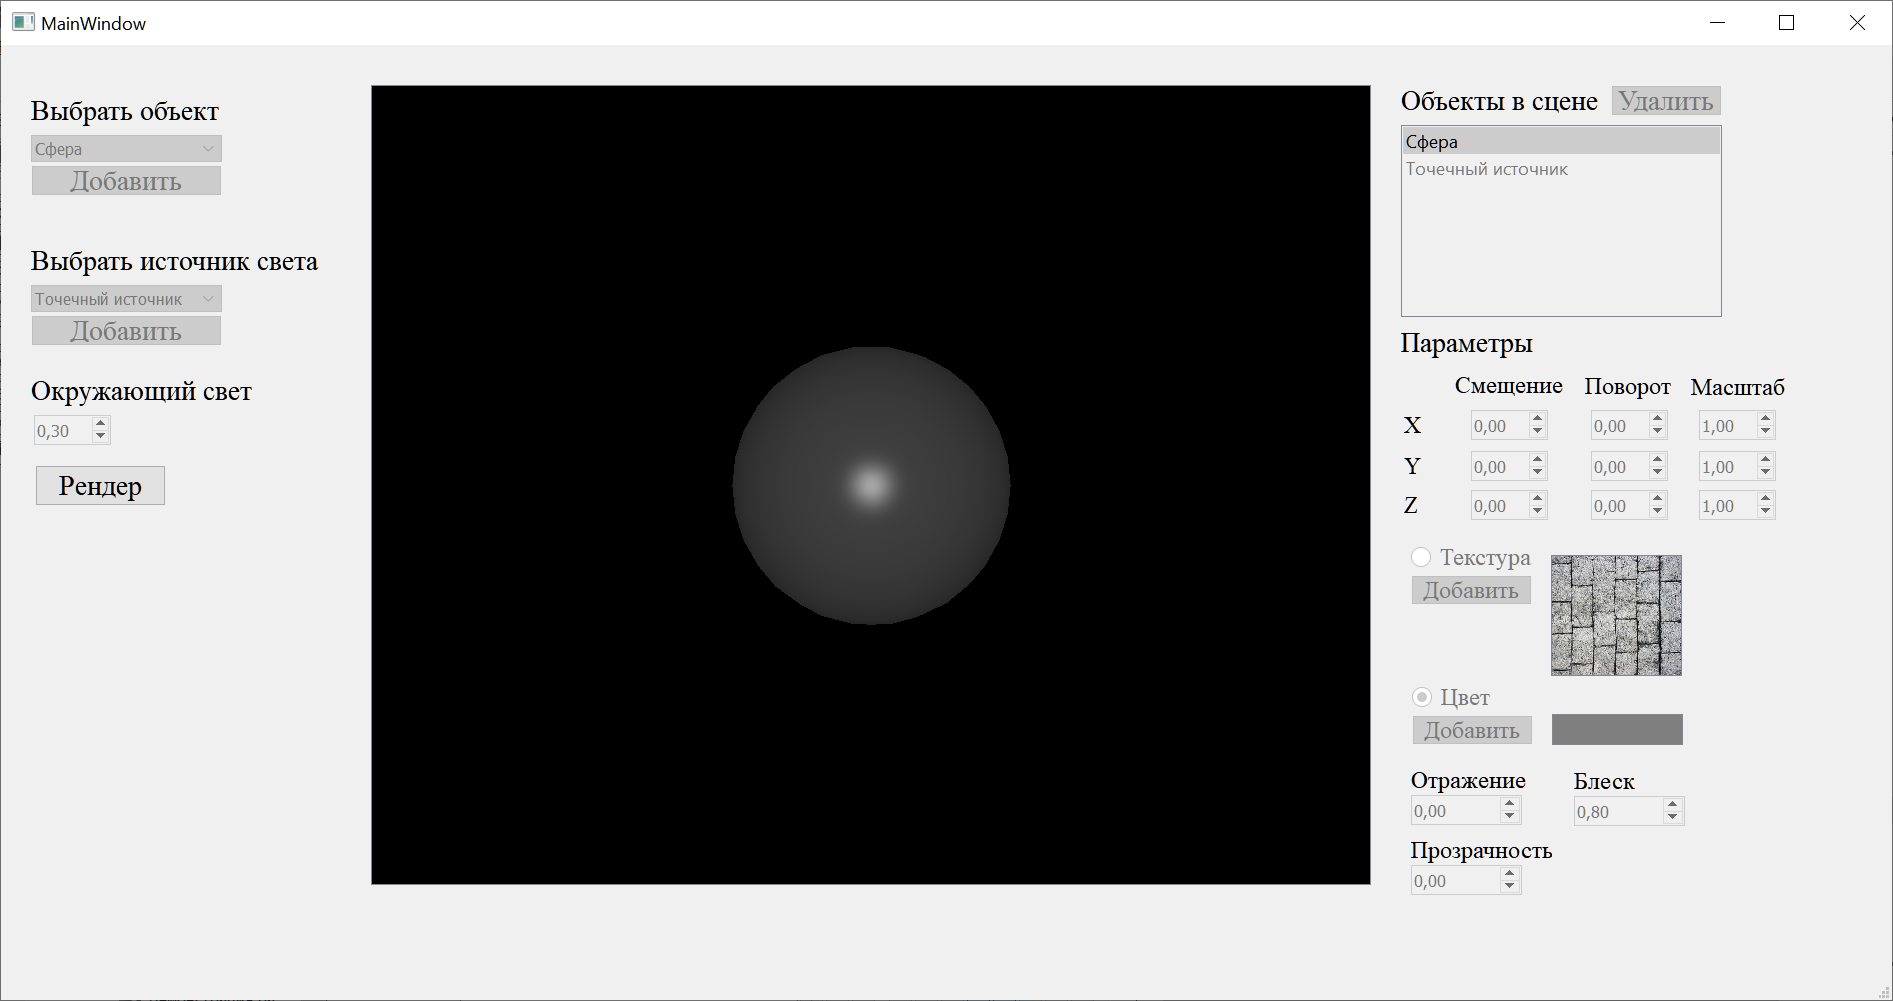
\includegraphics[scale = 0.5]{release}
		\caption{Результат рендеринга}
	\end{figure}
	
	
	\chapter{Исследовательский раздел}
	 \quad В алгоритме обратной трассировки лучи трассируются независимо друг от друга, это дает возможность проводить отрисовку изображения параллельно. Помимо этого прироста производительности можно достичь при использовании улучшений, призванных уменьшить количество обрабатываемых полигонов на каждом трассировании луча.
	
	Исследование проводится для поиска таких улучшений и определения числа потоков, при котором достигается минимальное время рендеринга сцены.
	
	
	\section{Технические характеристики}
	 \quad Технические характеристики устройства, на котором выполнялось тестирование:
	\begin{itemize}
		\item операционная система Windows 10, 64-bit;
		\item оперативная память 8 гб;
		\item intel(R) Core(TM) i5-7200U, 2 ядра, 4 логических процессора.
	\end{itemize}

	\section{Описание экспериментов}
	 \quad Для проведения замеров времени в экспериментах будет использована формула.
	
	\begin{equation}
	t = \frac{T_n}{N}
	\end{equation}
	
	где:
	\begin{conditions*}
		N & количество потоков,\\
		t & время выполнения реализации алгоритма,\\
		T_n & время выполнения N замеров
	\end{conditions*}

	 Неоднократное измерение времени необходимо для построения более гладкого графика и получения усредненного значения времени.
	
	\subsection{Зависимость времени работы алгоритма обратной трассировки лучей от количества потоков программы}
	
	 \quad Одним из преимуществ алгоритма обратной трассировки лучей является то, что его можно распараллелить, так как лучи не влияют на работу друг-друга и могут трассироваться параллельно\cite{t}.
	
	 На рисунке 4.1 изображен график зависимости рендеринга сцены, состоящей из конуса и куба с одним точечным источником света, от количества потоков.
	
	 Принцип разделения обязанностей был следюущим: картинка делилась на n частей по диагонали, где n - количество потоков. В итоге каждый поток получал строчку, в рамках которой и трассировал лучи.
	
	\begin{figure}[h]
		\centering
		\begin{tikzpicture}
		\begin{axis}[
		symbolic x coords={1, 2, 4, 8, 16},
		xtick=data,
		ylabel = {мс},
		xlabel = {количество потоков},
		]
		\addplot[ybar,fill=blue] coordinates {
			(1,   1266)
			(2,  798)
			(4,   584)
			(8,   590)
			(16,   600)
		};
		\end{axis}
		\end{tikzpicture}
		\caption{Диаграмма времени выполнения алгоритма в зависимости от количества потоков}
	\end{figure}
	
	 Как видно из рисунка, начиная с четырех, увеличение числа потоков не дало сильного прироста в скорости, это связано с тем, что число потоков, которые  работают параллельно, равно числу логических процессоров, которых на экспериментальном процессоре четыре.
	
	\subsection{Зависимость времени работы алгоритма обратной трассировки лучей от алгоритмов пересечения}
	
	 \quad Так как каждая модель состоит из полигонов, крайне неэффективно на каждом трассировании луча искать пересечение с объектом путем установления факта пересечения с его полигонами.
	
	 Для оптимизации можно использовать следующую идею: ограничить каждый объект параллелепипедом, который параллелен координатным осям (AABB -- axis-aligned bounding box). Таким образом при каждом трассировании луча пересечение будет вычисляться сначала с этим параллелепипедом (листинг 3.3), и если оно было найдено, то далее с полигонами этого объекта. 
	
	 На листинге 3.3 можно заметить, что операция обмена значений используется часто. Исходя из этого для дополнительной оптимизации имеет смысл заменить ее, предварительно вычислив обратное направление луча и знаки коориднат изначального вектора (листинг 3.4).
	
	 Наибольшее количество полигонов у модели сферы, поэтому эксперимент будет проводиться на ней (рисунок 4.2). Замеры проводились 5 раз при 4 потоках .
	
	
	\begin{figure}[h]
		\centering
		\begin{tikzpicture}
		\begin{axis}[
		symbolic x coords={Без AABB, AABB, Оптимизация AABB},
		xtick=data,
		ylabel = {с},
		xlabel = {алгоритм},
		]
		\addplot[ybar,fill=blue] coordinates {
			(Без AABB,   19)
			(AABB,  5)
			(Оптимизация AABB,   3)
		};
		\end{axis}
		\end{tikzpicture}
		\caption{Диаграмма времени отрисовки сферы в зависимости от алгоритма поиска пересечений луча с объектом}
	\end{figure}
	
	 Как видно из рисунка, использование AABB существенно ускоряет время работы программы, а применение ряда оптимизаций сокращает время отрисовки в среднем в 1.5 раза.
	
	\section{Демонстрация работы программы}
	 \quad На рисунках 4.3 и 4.4 представлены результаты работы программы.
	
	\begin{figure}[H]
		\centering
		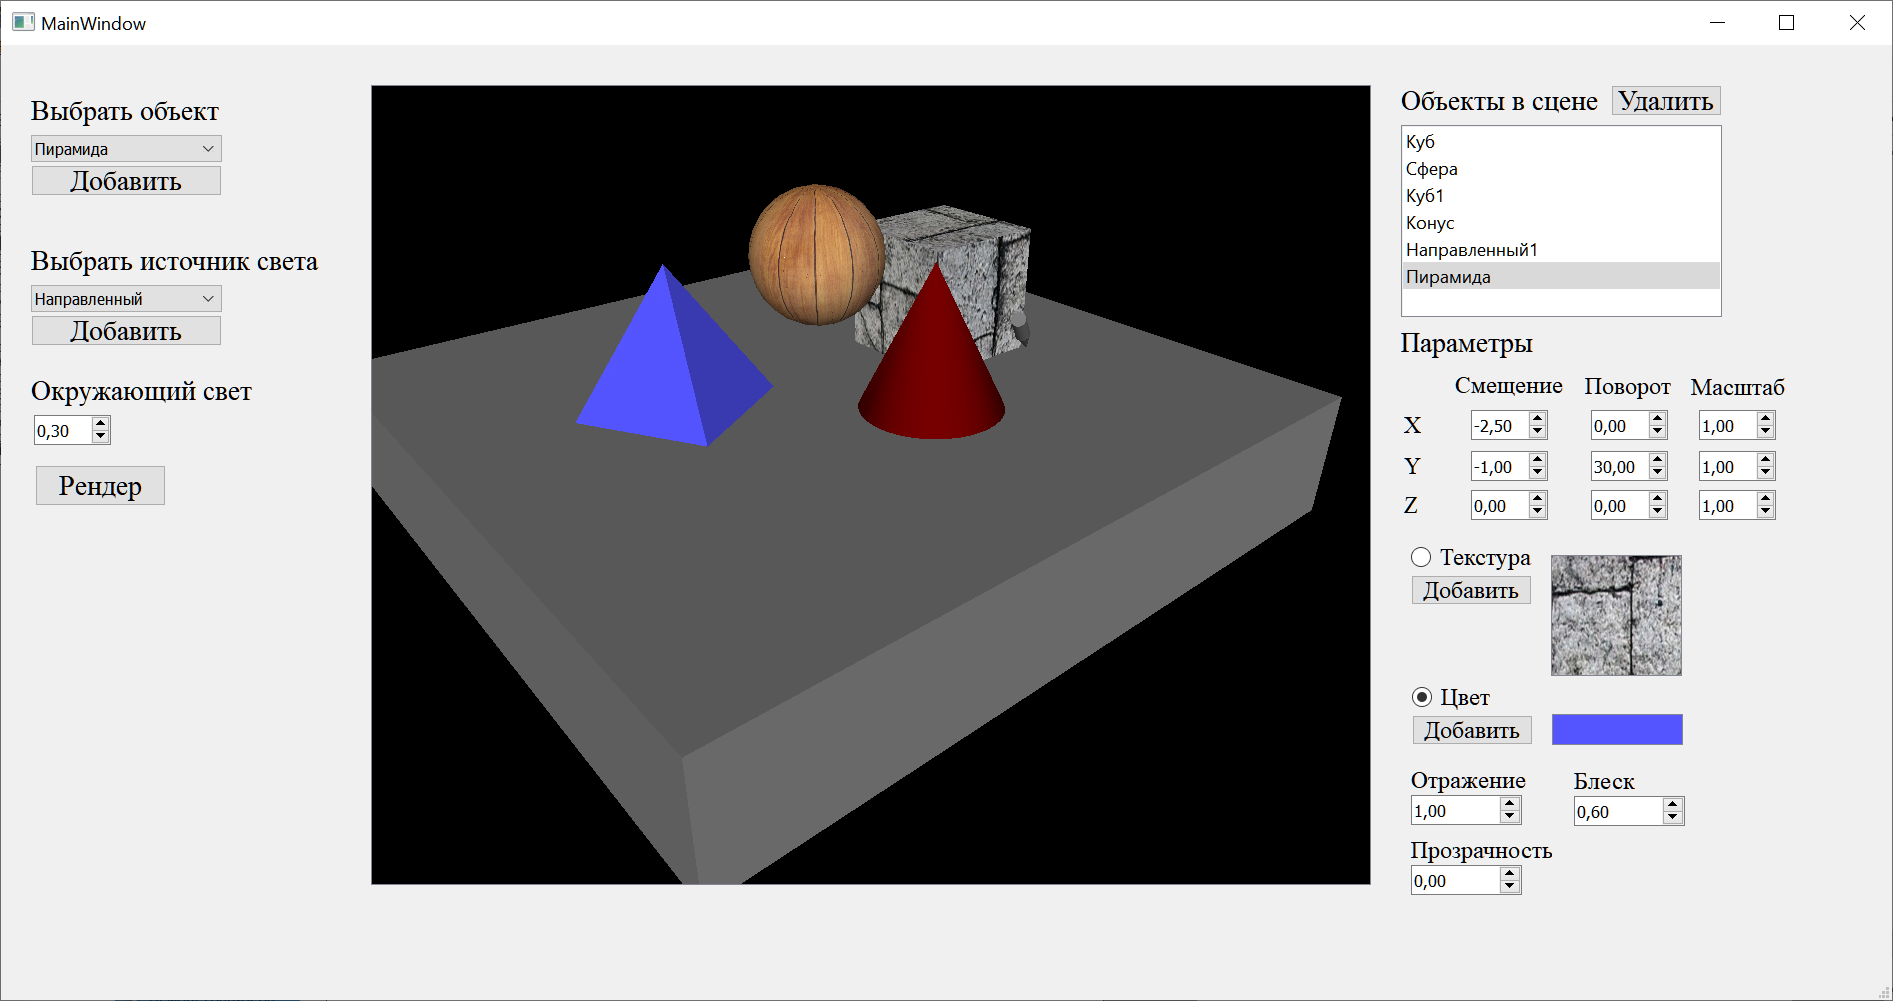
\includegraphics[scale = 0.5]{constructor}
		\caption{Созданная сцена в конструкторе}
	\end{figure}


	\begin{figure}[H]
		\centering
		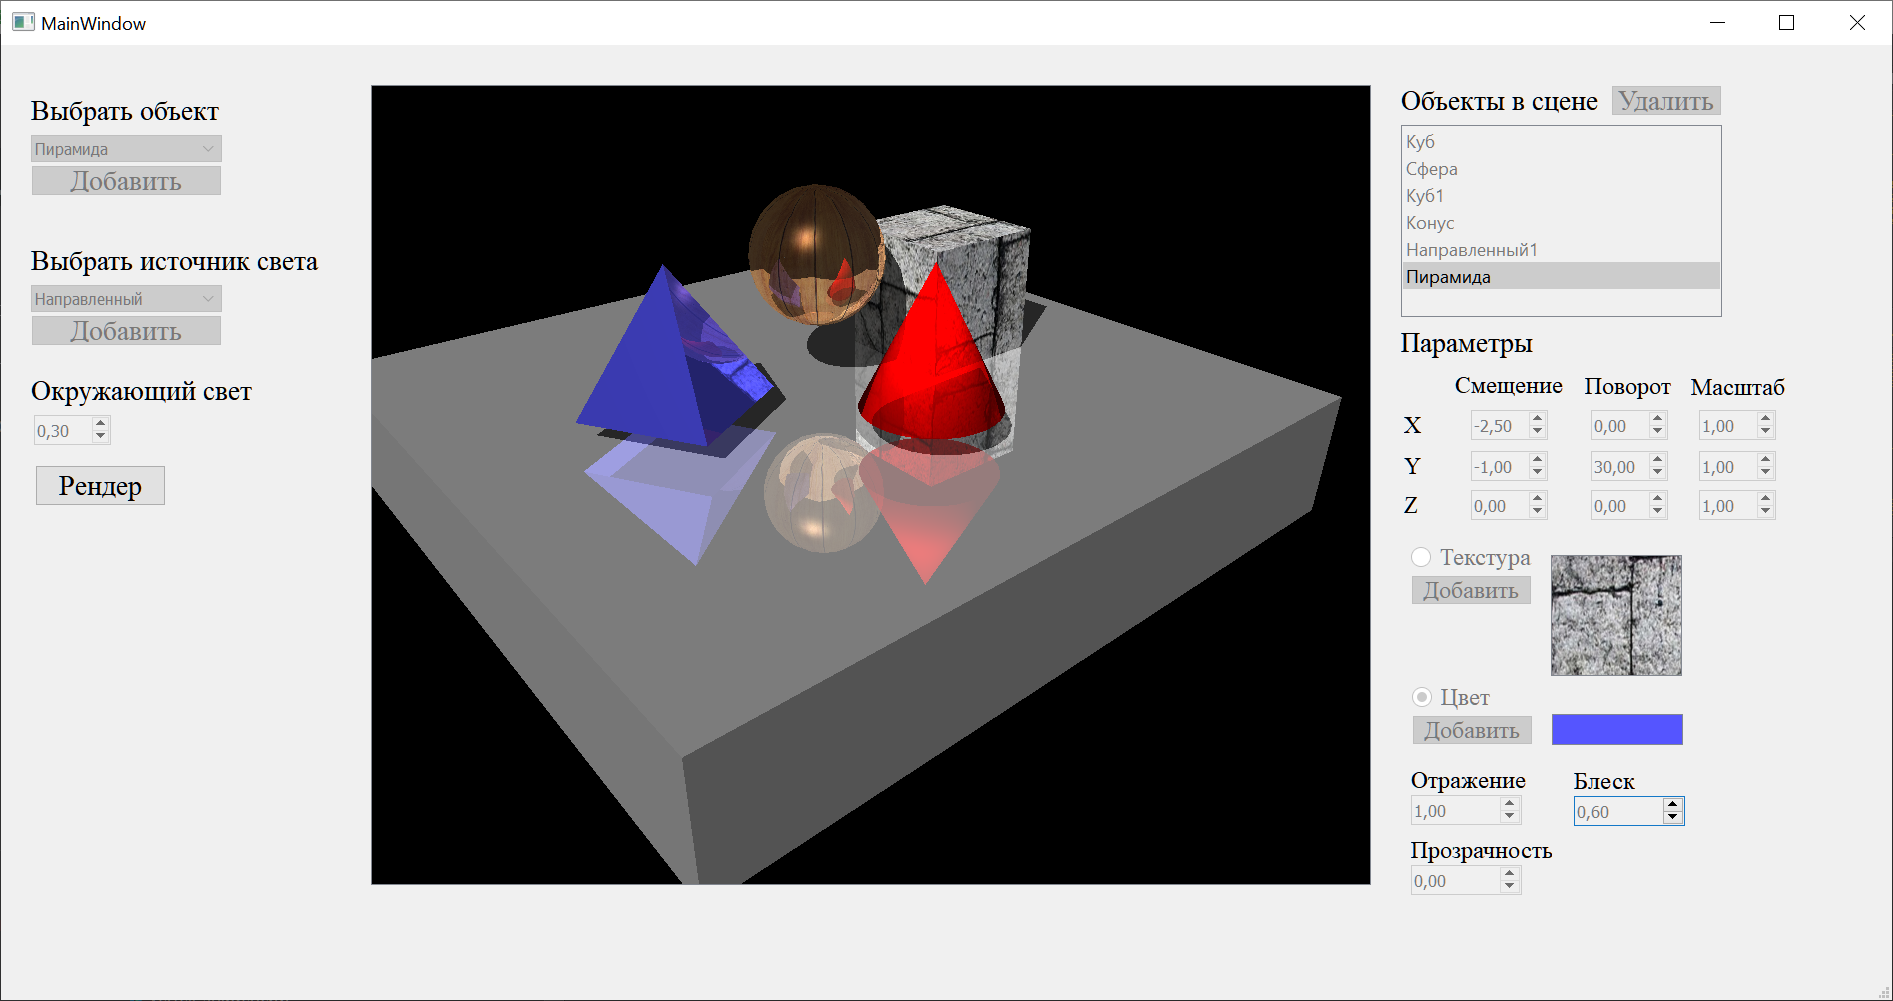
\includegraphics[scale = 0.5]{final}
		\caption{Построенное реалистическое изображение}
	\end{figure}
	

	\chapter*{Заключение}
	
	 \quad В рамках курсового проекта было создано программное обеспечение для создания графических сцен из готовых трехмерных моделей и их визуализации с учетом выбранной текстуры или цвета, а также оптических эффектов отражения, преломления, прозрачности, блеска. 
	
	 Были выполнены следующие задачи:
	\begin{itemize}
		\item проведен анализ существующих алгоритмов удаления невидимых линий и поверхностей, закраски, текстурирования, а также моделей освещения и выбраны подходящие для выполнения проекта;
		\item реализованы выбранные алгоритмы и структуры данных;
		\item разработано программное обеспечение, позволяющее отобразить трехмерную сцену;
		\item реализован интерфейс программного модуля;
		\item проведено исследование на основе разработанной программы. 
	\end{itemize}

	
	\addcontentsline{toc}{chapter}{Список использованной литературы}
	\renewcommand{\bibname}{Список использованной литературы}
	\begin{thebibliography}{2}
		\bibitem{f} Роджерс Д. Математические основы машинной графики. / Роджерс Д., Адамс Дж.  – М.: Мир, 1989. – 512с. 
		
		\bibitem{s} Аксенов, Андрей. Компьютерная графика.  [электронный ресурс]. Режим доступа:
		http://algolist.ru/graphics/3dfaq/index.php
		(Дата обращения: 16.12.2020)
		
		\bibitem{t} Проблемы трассировки лучей – из будущего в реальное время. [Электронный ресурс]. – Режим доступа: https://nvworld.ru/articles/ray-tracing/3/ (дата обращения 12.10.20) 
		
		\bibitem{four} RayTracing – царь света и теней, Лев Дымченко [Электронный ресурс]. – Режим доступа: https://old.computerra.ru/206167/ (дата обращения 14.10.20) 
			
	\end{thebibliography}
	
\end{document}